\documentclass[lettersize,journal]{IEEEtran}

\usepackage{amsmath,amsfonts}
\usepackage{algorithmic}
\usepackage{algorithm}
\usepackage{array}
\usepackage[caption=false, font=scriptsize, labelfont=rm, textfont=rm]{subfig}
\usepackage{textcomp}
\usepackage{stfloats}
\usepackage{url}
\usepackage{verbatim}
\usepackage{graphicx}
\usepackage{cite}
\usepackage{amsmath,amssymb,amsfonts}
\usepackage{graphicx}
\usepackage{textcomp}
\usepackage{xcolor}
\usepackage{booktabs}
\usepackage{multirow}
\usepackage{booktabs}  % 必须：用于画三线表
\usepackage{multirow}  % 用于合并单元格
\usepackage{xcolor}    % 用于高亮关键词
\usepackage{tabularx}  % 用于自动换行
\usepackage{amssymb}
\usepackage{hyperref}
\usepackage{url}

\hyphenation{op-tical net-works semi-conduc-tor IEEE-Xplore}
% updated with editorial comments 8/9/2021

\begin{document}

\title{LogICL: Distilling LLM Reasoning to Bridge the Semantic Gap in Cross-Domain Log Anomaly Detection}

\author{IEEE Publication Technology,~\IEEEmembership{Staff,~IEEE,}
        % <-this % stops a space
\thanks{This paper was produced by the IEEE Publication Technology Group. They are in Piscataway, NJ.}% <-this % stops a space
\thanks{Manuscript received April 19, 2021; revised August 16, 2021.}}

% The paper headers
\markboth{Journal of \LaTeX\ Class Files,~Vol.~14, No.~8, August~2021}%
{Shell \MakeLowercase{\textit{et al.}}: A Sample Article Using IEEEtran.cls for IEEE Journals}

\IEEEpubid{0000--0000/00\$00.00~\copyright~2021 IEEE}
% Remember, if you use this you must call \IEEEpubidadjcol in the second
% column for its text to clear the IEEEpubid mark.

\maketitle

\begin{abstract}
%-------------------------------原版字数超过-------------------------------------
% Automated log anomaly detection is pivotal for ensuring the reliability of large-scale IT infrastructures. While Transformer-based models have established a new paradigm, However, these models impose high computational demands and require substantial labeled data for pre-training or fine-tuning, exacerbating the cold-start problem in target domains where logs are scarce due to system evolution. To mitigate data scarcity, cross-domain transfer learning methods leverage source-domain logs, However, existing methods primarily rely on Surface Lexical Similarity, failing to capture latent semantic equivalence amid structural and terminological divergences across heterogeneous systems. To concurrently address these limitations, we propose LogICL, a framework that distills LLM reasoning into a lightweight log sequence encoder for effective cross-domain anomaly detection. During offline training, LogICL constructs a sparse Delta Matrix by assessing LLM zero-shot and one-shot performance on demonstrations selected via Maximal Marginal Relevance, the encoder is jointly optimized with a multi-objective loss that includes an ICL-guided term—pulling together representations of source-target pairs with positive reasoning assistance while pushing apart interfering pairs in the representation space—alongside maximum mean discrepancy for domain alignment and supervised contrastive loss for anomaly discrimination. During inference, the optimized encoder retrieves reasoning-aware demonstrations based on semantic similarity and delta scores to facilitate In-Context Learning (ICL) with a frozen LLM, employing Chain-of-Thought reasoning to enhance detection accuracy while providing interpretable diagnostics. 

% Experiments on few-shot and zero-shot cross-domain benchmarks show that LogICL achieves state-of-the-art performance, outperforming existing LLM-based and transfer learning baselines. Further analyses, including visualization of the learned alignment mechanisms and case studies of retrieved demonstrations, confirm that LogICL effectively identifies source-domain samples that provide genuine reasoning benefits to the target domain, thereby bridging the cross-domain semantic gap beyond surface lexical similarity and achieving robust capture of latent semantic equivalence for rapid deployment in new systems.
%-------------------------------原版字数超过-------------------------------------

Effective log anomaly detection is critical to sustaining reliability in large-scale IT infrastructures. Transformer-based language models have advanced the field but require substantial computational resources and labeled data, exacerbating the cold-start problem in target domains where logs are scarce due to system evolution.
Cross-domain methods alleviate data scarcity by leveraging source domain logs. However, their reliance on surface lexical similarity limits cross-domain generalization, as they fail to capture latent semantic equivalence amid structural and terminological divergences.

To address these challenges, we propose LogICL, a framework that distills Large Language Model (LLM) reasoning into a lightweight encoder for cross-domain anomaly detection. 
% During training, LogICL builds a delta matrix by evaluating LLM zero-shot and one-shot performance on demonstrations selected via Maximal Marginal Relevance. 
During training, LogICL constructs a delta matrix by measuring the utility of demonstrations selected via Maximal Marginal Relevance algorithm relative to zero-shot inference.
The encoder is jointly optimized via a multi-objective loss comprising an ICL-Guided term that pulls together representations of source-target pairs with positive reasoning assistance while pushing apart interfering pairs in the representation space, maximum mean discrepancy for domain alignment, and supervised contrastive loss for anomaly discrimination. At inference, the optimized encoder retrieves reasoning-aware demonstrations based on semantic similarity and delta scores, enabling frozen-LLM in-context learning with chain-of-thought reasoning for accurate and interpretable anomaly detection.

% Experiments on few-shot and zero-shot cross-domain benchmarks show that LogICL achieves state-of-the-art performance, outperforming existing LLM-based and transfer learning baselines. 
Experiments on few-shot and zero-shot cross-domain benchmarks confirm that LogICL achieves state-of-the-art performance across heterogeneous log systems.
Further experimental validation via alignment visualizations and case studies confirms that LogICL bridges the semantic gap beyond surface lexical similarity, effectively capturing latent semantic equivalence for rapid deployment in new systems.
% Visualizations of alignment mechanisms and case studies of retrieved demonstrations further confirm that LogICL bridges the semantic gap beyond surface lexical similarity, effectively capturing latent semantic equivalence for rapid deployment in new systems.

\end{abstract}

\begin{IEEEkeywords}
Log anomaly detection, Cross domain, In-context learning, Latent semantic equivalence, Large language model.
\end{IEEEkeywords}

\section{Introduction}
% Modern large-scale software systems, such as distributed platforms, cloud services, and enterprise infrastructures, generate massive amounts of log data that record system operations, component interactions, and runtime states. These logs serve as a critical foundation for ensuring system reliability and provide valuable insights into performance degradation, service failures, and security anomalies. 
Modern large-scale software systems—including distributed platforms, cloud services, and enterprise infrastructures—produce massive volumes of logs that capture system operations, component interactions, and runtime states. As a primary source of observability, these logs are instrumental for maintaining system reliability and play a central role in diagnosing performance degradation, identifying service failures, and detecting anomalies. Consequently, effective log analysis is essential for ensuring the robustness and trustworthiness of modern computing systems.

Log-based anomaly detection has therefore become an indispensable technique for maintaining stable and dependable software operations, enabling timely identification and diagnosis of abnormal behaviors before they escalate into severe system disruptions~\cite{chalapathy2019deep,he2021survey,he2016experience}. 

In recent years, Transformer-based language models have established a new paradigm in log anomaly detection, broadly categorized into Language Models (LMs) and Large Language Models (LLMs). LM-based approaches (e.g., LogBERT~\cite{guo2021logbert}, NeuralLog~\cite{chen2021neurallog}, LogOW~\cite{ye2025logow}) leverage masked language modeling and contextual embeddings to capture stable token-level patterns, enabling robust anomaly scoring with modest supervision. More recently, LLM-based methods (e.g., LogGPT~\cite{han2023loggpt}, LogLLM~\cite{guan2024logllm}) have demonstrated remarkable capabilities in reasoning and few-shot generalization, utilizing high-capacity encoders and extensive pre-training to model complex, long-range log dependencies across diverse formats.

% However, the efficacy of these Transformer-based architectures comes at a significant cost. Both LMs and LLMs demand substantial computational resources and large-scale, high-quality datasets for pre-training or fine-tuning. While LLMs exhibit superior few-shot performance, their massive parameter scale introduces high latency and deployment costs. Even relatively smaller LMs require considerable training overhead compared to lightweight statistical methods, limiting their feasibility in resource-constrained or real-time operational environments. 
However, these Transformer-based approaches achieve high accuracy and generalization at a substantial cost: both LMs and LLMs rely heavily on large-scale, high-quality labeled datasets for effective pre-training or fine-tuning. In the absence of sufficient labeled data—which is common in new or cross-domain deployments—their performance degrades sharply. Moreover, their substantial parameter counts and training requirements impose significantly higher computational overhead than lightweight statistical or deep-log parsers, rendering them impractical when labeled logs are scarce or computational resources are limited.
This challenge is further exacerbated by the rapid evolution of modern software systems~\cite{torrey2010transfer, ye2025logow}. The scarcity of labeled logs in target systems renders the supervised training of data-intensive Transformer-based log anomaly detection models infeasible~\cite{ye2025logow}. 

To address data scarcity, cross-system methods attempt to transfer knowledge from high-resource source domains to target domains. LogTransfer~\cite{chen2020logtransfer} utilizes shared layers with GloVe embeddings; LogTAD~\cite{han2021unsupervised} employs adversarial domain adaptation technique training for cross domain; and MetaLog~\cite{zhang2024metalog} applies meta-learning to construct shared semantic spaces.

Despite existing methods have achieved preliminary success in mitigating data scarcity, they continue to face significant challenges in cross-domain scenarios. These challenges can be summarized in two key areas:

\IEEEpubidadjcol

\paragraph{Inadequate Capture of Latent Semantic Equivalence across Domains}
% \textbf{(1) Inadequate Capture of Latent Semantic Equivalence across Domains.} 
Existing transfer learning-based log anomaly detection methods predominantly utilize static pre-trained word embeddings for feature extraction. Consequently, these approaches primarily capture \textit{surface lexical similarity}, failing to model \textit{latent semantic equivalence} across heterogeneous log systems. As illustrated in Figure~\ref{Lexical-Semantic Similarity & Semantic Equivalence}, consider a cross-system scenario where the source domain log message (Thunderbird) and target domain log message (HDFS) both record a critical \textit{Network Transmission Failure}. To a human expert, these logs convey identical operational intelligence, yet their manifestations diverge fundamentally across three semantic dimensions: \textit{Action}, \textit{Outcome}, and \textit{Root Cause}.

Figure \ref{Lexical-Semantic Similarity & Semantic Equivalence} illustrates the key challenge in cross-domain log anomaly detection through two representative examples, highlighting the distinction between surface lexical similarity and latent semantic equivalence.
The upper part of Figure 1 demonstrates a case of strong surface lexical similarity with structural and logical alignment. Logs from the Thunderbird (source) and BGL (target) domains share highly similar syntactic templates—both follow a component-action-outcome-reason structure—and employ nearly identical failure-related vocabulary (e.g., ``FATAL'' ``failed'', and the exact POSIX error ``No such file or directory''). This high lexical and structural overlap enables traditional methods relying on static word embeddings or n-gram matching to effectively capture the correspondence, facilitating positive transfer across domains.
In contrast, the lower part of Figure 1 presents a scenario of latent semantic equivalence masked by structural and logical divergence. Although logs from the Thunderbird (source) and HDFS (target) domains describe the same root cause (``Connection reset by peer'' vs. ``Connection refused''), they exhibit fundamentally different syntactic organizations: the source uses a procedural narrative centered on actions and exceptions, while the target adopts a declarative key-value state description. Compounded by substantial lexical discrepancy (e.g., ``transfer blk'' vs. ``relay'' ``sendmail''), conventional approaches based on surface-level features misinterpret these semantically equivalent anomalies as unrelated, resulting in severe negative transfer and degraded detection performance.
These contrasting cases underscore a critical limitation of existing methods: their heavy reliance on superficial lexical and structural cues hinders the capture of deeper semantic equivalence across diverse log domains, significantly impairing cross-domain generalization—particularly in few-shot settings with limited target-domain supervision.

% %图1的上部分解释%
% First, referring to the upper part of Figure 1, the logs from the source and target domains exhibit Structural and Logical Alignment. The Thunderbird (source domain) log follows a \textit{Standard Error Reporting} structure (\textit{modprobe: FATAL: Could not load ...}). It employs a linear logic: the \textit{Component} (\textit{modprobe}) declares a \textit{Severity} (\textit{FATAL}) and an \textit{Action Failure} (\textit{Could not load...}), followed by the \textit{Reason} (\textit{No such file or directory}). Similarly, the BGL (target domain) adopts a congruent \textit{Component-Action-Status} structure (\textit{ciod: LOGIN ... failed: ...}). Here, the semantics follow an identical procedural flow: the \textit{Component} (\textit{ciod}) initiates an \textit{Action} (\textit{LOGIN}) that results in a \textit{Negative Outcome} (\textit{failed}), culminating in the same \textit{Reason} appended after the colon. This shared syntactic template creates a structural bridge that facilitates direct pattern mapping across domains.

% Second, this alignment is reinforced by High Lexical Similarity. Even at the token level, the domains express the root cause using identical vocabulary. Both the source and target logs conclude with the exact POSIX error string: ``\textit{No such file or directory}''. Furthermore, the functional keywords indicating failure (\textit{Could not load} and \textit{failed}) are semantically equivalent and positionally consistent. Consequently, traditional methods relying on static word embeddings or n-gram matching can easily capture this surface-level overlap, enabling effective positive transfer without requiring deep semantic reasoning.

% %图1的下部分解释
% First, referring to the lower part of Figure \ref{Lexical-Semantic Similarity & Semantic Equivalence}, the logs from different domains exhibit \textbf{Structural and Logical Divergence}. The Thunderbird (source domain) follows a \textit{Causal Narrative} structure (\textit{Failed to transfer blk\_\textless\textgreater\ to \textless\textgreater\ got java.io.IOException...}). It employs a linear logic: the \textit{Action} is an attempted block transmission (\textit{transfer blk}); the \textit{Outcome} is an explicit failure (\textit{Failed}); and the \textit{Root Cause} is a specific exception (\textit{Connection reset by peer}). In contrast, the HDFS (target domain) adopts a \textit{State-Attribute Declaration} structure using disjoint key-value pairs (\textit{mailer=relay ... stat=Deferred: Connection refused by [\textless\textgreater]}). Here, the semantics are encoded as static attributes: the \textit{Action} is defined by a service parameter (\textit{relay}); the \textit{Outcome} is encoded as a system state (\textit{Deferred}); and the \textit{Root Cause} is appended as a status detail (\textit{Connection refused}). This shift from a procedural narrative to a declarative state creates a structural chasm that sequential models fail to bridge.

% Second, this is compounded by \textbf{Lexical Discrepancy}. Even at the token level, the domains express identical concepts through disjoint vocabularies. The source domain log utilizes generic file-system terminology like \textit{transfer} and \textit{blk}, whereas the target domain log employs protocol-specific jargon such as \textit{relay} and \textit{sendmail}. Consequently, traditional methods interpret this structural orthogonality and terminological mismatch as semantic distinctness, leading to negative transfer.

% \textbf{(2) High Computational and Data Constraints of Language Models.}
\paragraph{High Computational and Data Constraints of Language Models}
While Transformer-based models offer superior performance, their deployment is hindered by excessive resource demands. This constraint applies not only to massive LLMs but also to BERT-based LMs, which still require significant computational power for fine-tuning and inference compared to traditional methods. The dependence on high-quality labeled datasets further complicates their application in real-world environments where data is noisy or scarce. Even with efficient tuning strategies (e.g., LoRA), the fundamental trade-off between model capacity and resource efficiency remains a persistent hurdle for scalable log analysis.

\begin{figure}[htbp]
\centerline{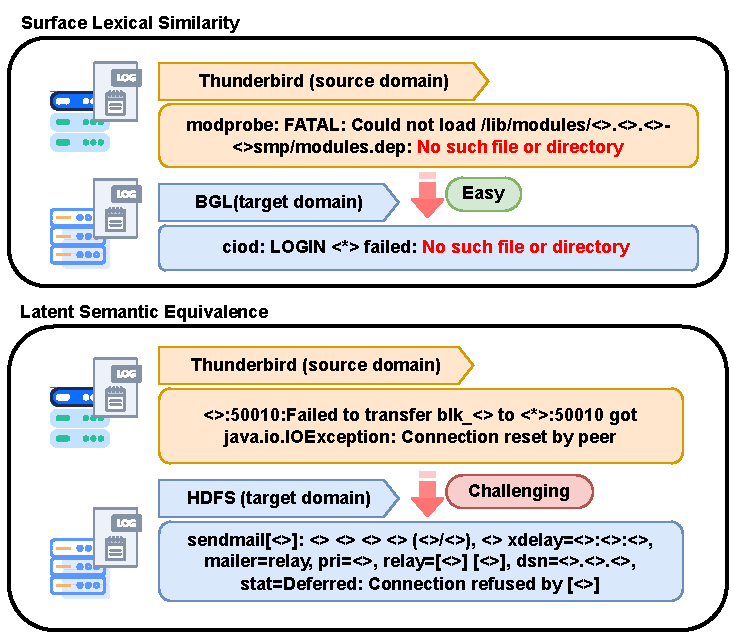
\includegraphics[scale=0.7]{Figures/Surface Lexical Similarity & Latent Semantic Equivalence.pdf}}
\caption{Surface Lexical Similarity \& Latent Semantic Equivalence.}
\label{Lexical-Semantic Similarity & Semantic Equivalence}
\end{figure}

% To resolve the limitations outlined above, we propose LogICL, a framework that leverages in-context learning (ICL) for improved cross-domain generalization. Specifically, LogICL addresses two critical challenges: (1) inadequate modeling of semantic equivalence across logs with varying structures and terminology, and (2) the high computational and data demands of large language models (LLMs), which typically require extensive fine-tuning and labeled datasets. In summary, this paper makes the following contributions:

In summary, to address the aforementioned limitations, we propose LogICL, a novel framework that harnesses ICL to enhance cross-domain generalization and detection accuracy in few-shot log anomaly detection settings with scarce target-domain supervision.
Specifically, LogICL tackles two key challenges: (1) the inadequate modeling of latent semantic equivalence across heterogeneous logs with varying structures and terminology; and (2) the substantial computational and data requirements of LMs, which often rely on resource-intensive training paradigms and abundant labeled data. The main contributions of this paper can be summarized as follows:

\begin{itemize}

\item We propose LogICL, a novel log anomaly detection framework that integrates ICL as a key component. It introduces a reasoning-guided, representation-aware demonstration selection paradigm that leverages LLM reasoning feedback to refine the encoder and identify demonstrations most beneficial for downstream inference. This mechanism enables the model to generalize effectively under data-scarce target domains without requiring updates to LLM parameters, allowing LogICL to surpass existing log anomaly detection methods in both few-shot and zero-shot scenarios.

\item We propose LogICL, which enhances cross-domain knowledge transfer by leveraging the causal reasoning capabilities of large models. It aligns logs describing similar events with different phrasing and structures, extracting shared knowledge across domains. This enables more accurate anomaly detection in heterogeneous environments, facilitating robust log analysis across diverse systems and improving detection performance.
\end{itemize}

\section{Preliminaries and Related Work}
\subsection{Preliminaries}

% \begin{figure}[htbp]
%     \centering
%     % 建议使用 width=0.X\linewidth 来控制大小，比 scale 更稳健
%     % 如果想保持原大小，可以调整 0.8 这个数值
%     \includegraphics[width=0.8\linewidth]{Figures/f2_transfer_learning.pdf}
    
%     % IEEE 格式：标题结尾通常加句号（虽然系统会自动处理，但写全比较好）
%     \caption{Cross Domain Knowledge Transfer.} 
%     \label{tl}
% \end{figure}

% Transfer learning (TL) aims to enhance model performance in target domains with limited labeled data by leveraging knowledge from related source domains with sufficient data \cite{weiss2016survey,zhuang2020comprehensive,tan2018survey,torrey2010transfer}. TL transfers useful and generalizable knowledge from the source domain to the target domain, enabling effective learning even under data scarcity. Unlike conventional supervised learning, which assumes identical data distributions, TL allows knowledge sharing across domains with different feature or label spaces. Existing TL methods are generally classified into three categories. Instance-based approaches reweight or select source samples to better match the target distribution, emphasizing transferable instances while reducing the influence of dissimilar ones. Feature-based approaches learn domain-invariant representations by mapping source and target data into a shared feature space through techniques such as moment matching, adversarial alignment, or distribution normalization. Model-based approaches reuse parameters or architectures from pre-trained models, enabling efficient adaptation to new domains via fine-tuning or parameter regularization. Collectively, these strategies form the foundation of transfer learning, supporting effective knowledge reuse and improving cross-domain generalization in data-scarce environments.

Transfer Learning (TL) constitutes a machine learning paradigm designed to improve generalization in a target domain by leveraging knowledge acquired from related source domains \cite{weiss2016survey,zhuang2020comprehensive}. Fundamentally, TL relaxes the independent and identically distributed (i.i.d.) assumption inherent in traditional supervised learning, enabling effective model adaptation across domains with shifting distributions or disparate feature spaces, particularly under supervision scarcity \cite{DBLP:journals/tkde/PanY10}. Existing methodologies are generally categorized into three paradigms: (1) Instance-based approaches, which mitigate distribution mismatch (e.g., covariate shift) by reweighting or selecting source samples that structurally resemble target instances; (2) Feature-based approaches, which project source and target data into a shared, domain-invariant latent space to align marginal or conditional distributions; and (3) Model-based approaches, which transfer structural knowledge or inductive biases by reusing pre-trained parameters and architectures to accelerate downstream adaptation.

\begin{figure}[htbp]
\centerline{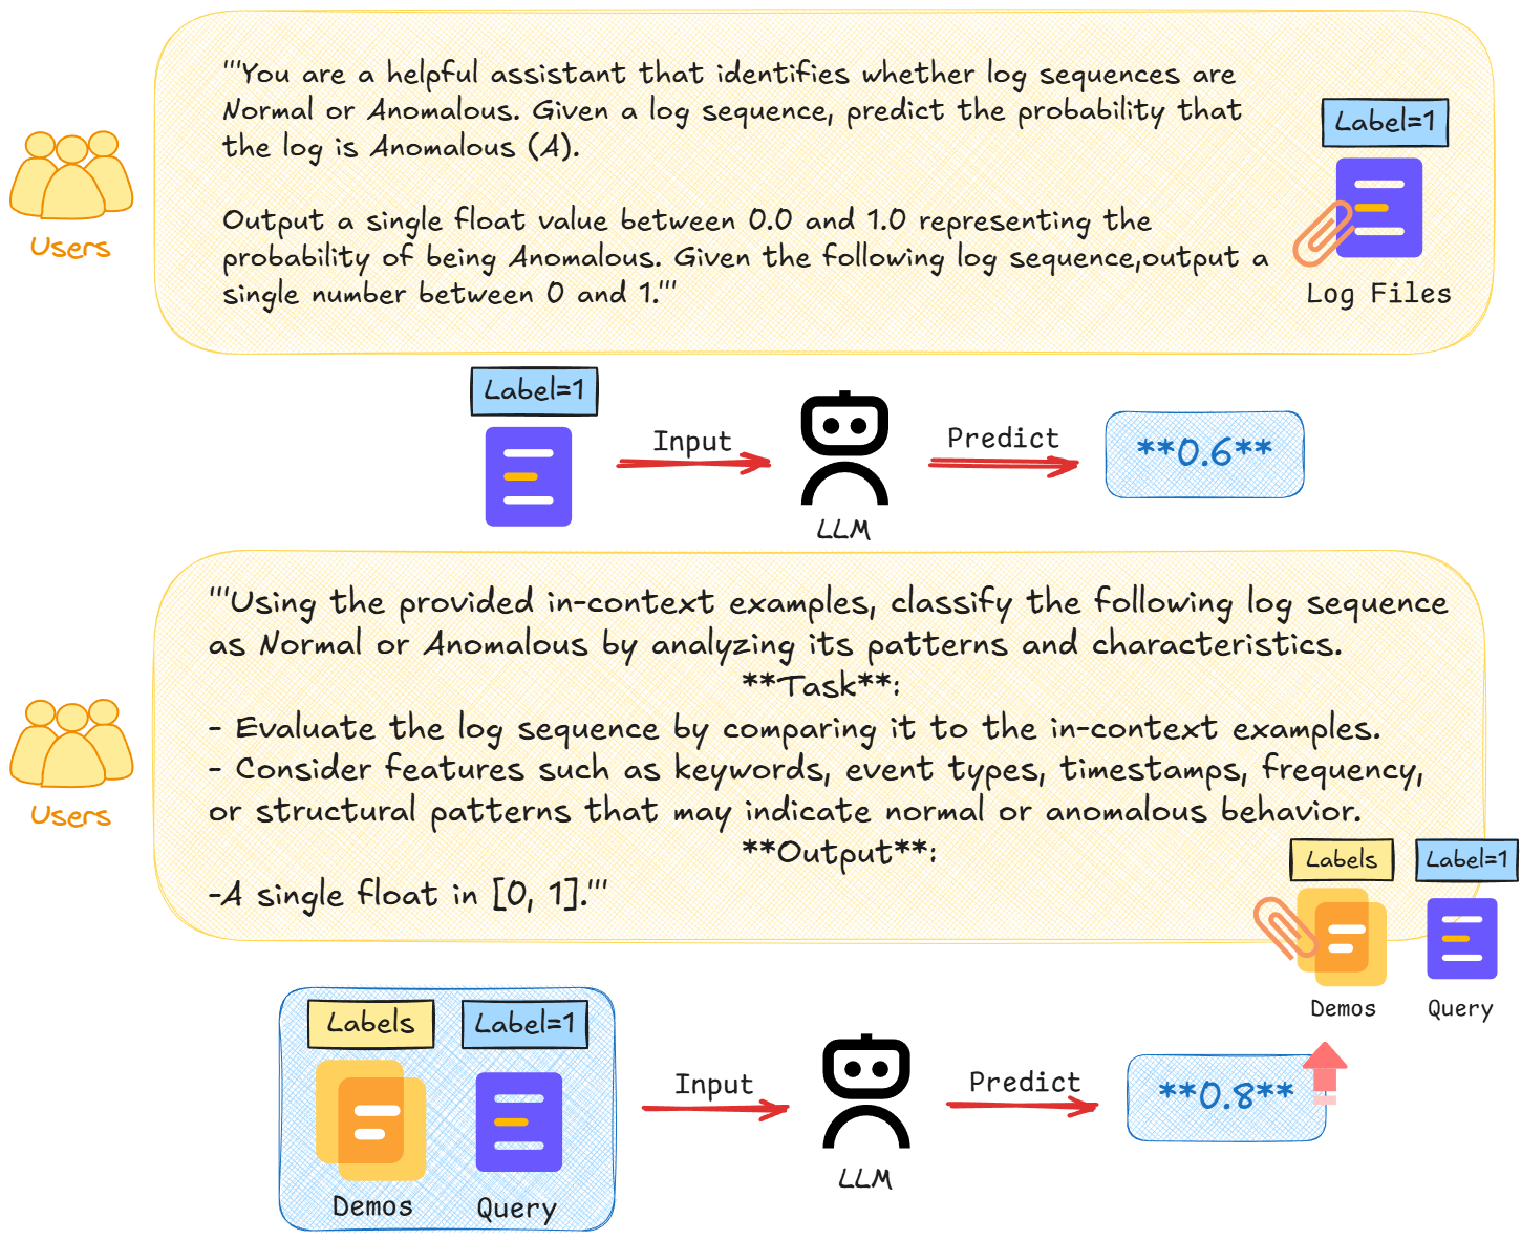
\includegraphics[scale=0.35]{Figures/ICL_anomaly_detection.pdf}}
\caption{In-context learning example for log anomaly detection.}
\label{fig:In_context_learning_for_Log_Anomaly_Detection}
\end{figure}

In-Context Learning (ICL) enables Large Language Models (LLMs) to adapt to downstream tasks by conditioning on demonstrations within the context window, effectively bypassing parameter updates \cite{brown2020language}. Unlike gradient-based fine-tuning, ICL operates via inference-time pattern recognition, where performance is highly sensitive to the selection, ordering, and formatting of demonstrations \cite{dong2022survey}. Theoretically, this mechanism has been formalized as implicit Bayesian inference or meta-optimization driven by attention dynamics \cite{xie2021explanation,falck2024context}. Consequently, ICL facilitates robust few-shot generalization, bridging the gap between pre-training and downstream deployment in low-resource settings. Fig.~\ref{fig:In_context_learning_for_Log_Anomaly_Detection} demonstrates the effectiveness of ICL for log analysis. While standard prompting often yields suboptimal performance on complex log patterns, ICL enhances the results by introducing reference examples. As illustrated, when an LLM analyzes a log query directly, the detection accuracy is often limited. To address this, relevant samples are selected to serve as in-context demonstrations. By providing these demonstrations alongside the query, the LLM utilizes the context to output a more accurate prediction.

\subsection{Related Work}

The traditional log anomaly detection pipeline, as illustrated in Fig.~\ref{workflow_log_anomaly_detection}, typically consists of six stages: (1) log collection (2) preprocessing raw log messages to remove erroneous identifiers and incomplete logs; (3) log parsing to convert unstructured text into structured event templates; (4) log grouping to form context-aware sequences (e.g., by session or time); (5) feature extraction to transform textual data into vector representations; and (6) anomaly detection by training learning-based models on these vectors to identify anomalies.

\begin{figure}[htbp]
\centerline{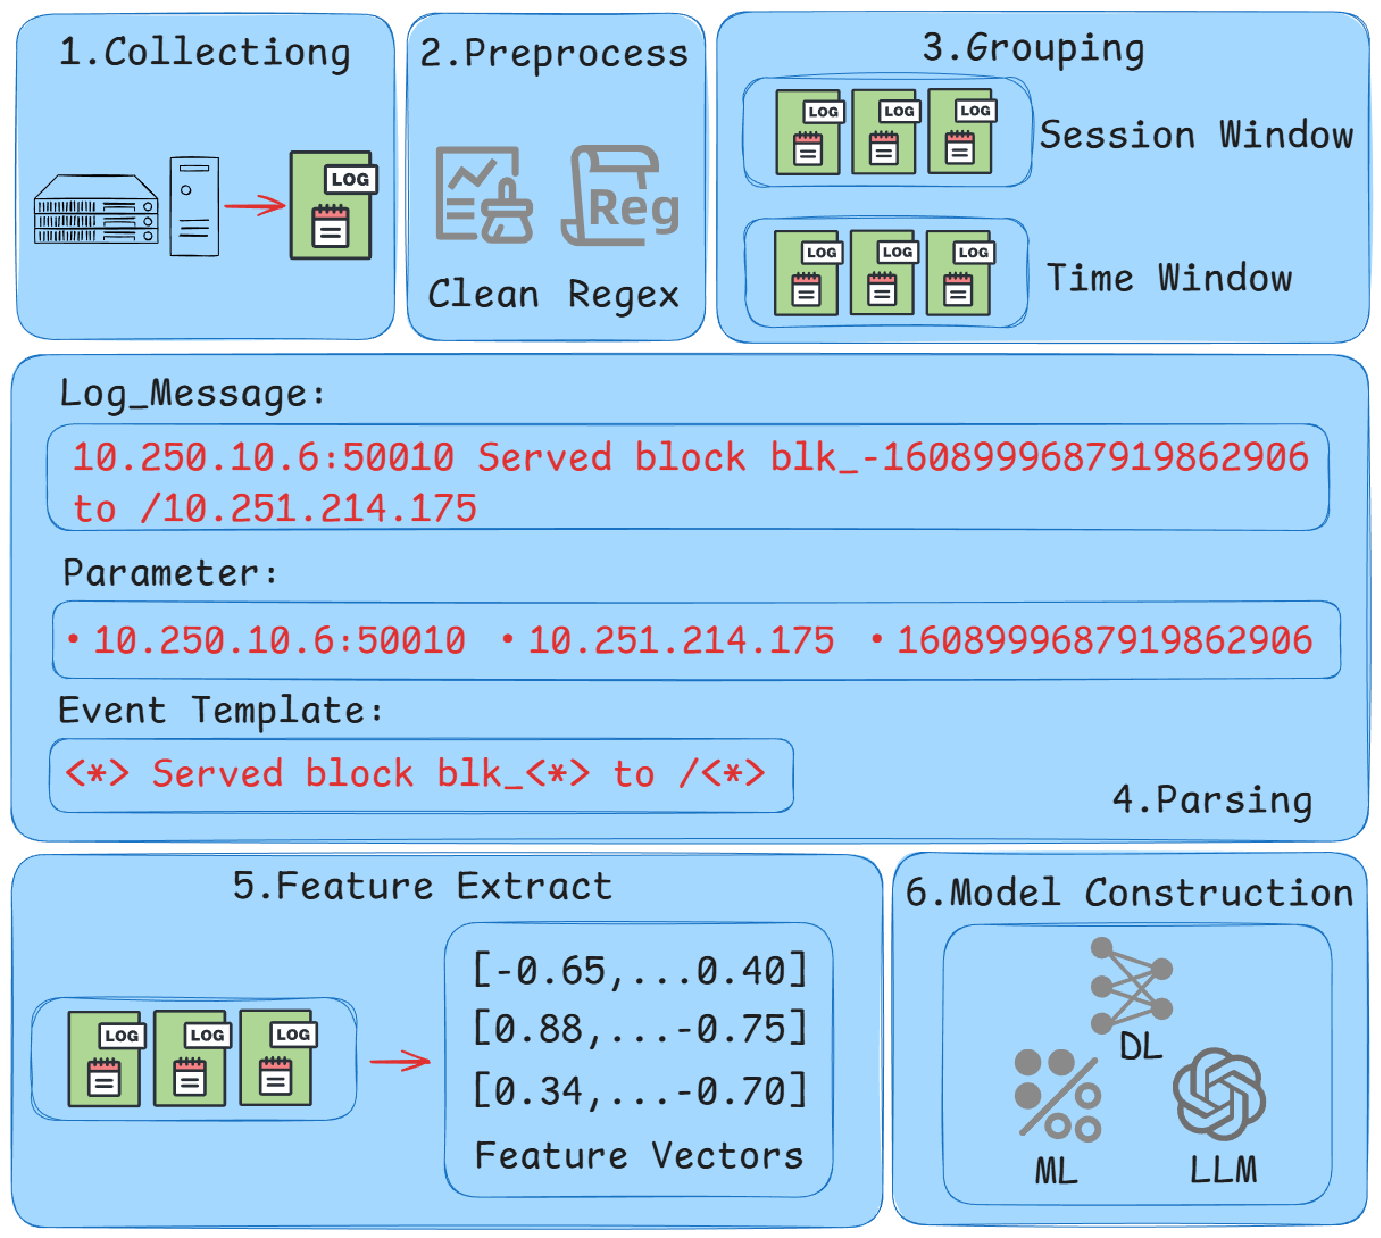
\includegraphics[scale=0.35]{Figures/pipline of logAD.pdf}}
\caption{Traditional workflow of log anomaly detection.}
\label{workflow_log_anomaly_detection}
\end{figure}

In recent years, LLMs have attracted growing interest in log anomaly detection. In the log parsing stage, approaches such as LLMParser~\cite{ma2024llmparser}, LogPrompt, and LogRules~\cite{huang2025logrules} leverage LLMs—either through fine-tuning or prompting—to extract structured event templates from raw log messages. In the anomaly detection stage, existing methods can be broadly classified into two categories: parameter-freezing and parameter-tuning approaches. Parameter-freezing methods, including FlexLog~\cite{hadadi2025llm}, LogPrompt, LogRules, EagerLog~\cite{duan2025eagerlog}, and LogRAG, rely on the generalization ability of pretrained LLMs while keeping all model parameters frozen. In contrast, parameter-tuning (fine-tuning-based) methods—such as LogGPT~\cite{han2023loggpt}, LogLLM~\cite{guan2024logllm}, SuperLog~\cite{ji2024adapting}, NLPLog~\cite{ji2024adapting}, and RationAnomaly~\cite{xu2025rationanomaly}—adapt LLMs to log-specific tasks by updating model parameters.

Our work addresses the cold-start scenario characterized by scarce source domain data and the resulting semantic gap. By retrieving optimal demonstrations to facilitate ICL with a frozen LLM, our framework bridges the cross-domain gap without parameter optimization. This strategy efficiently harnesses the model's generalization capabilities for zero-shot and few-shot anomaly detection.

\section{Design of Model}

\begin{figure*}[htbp]
\centering
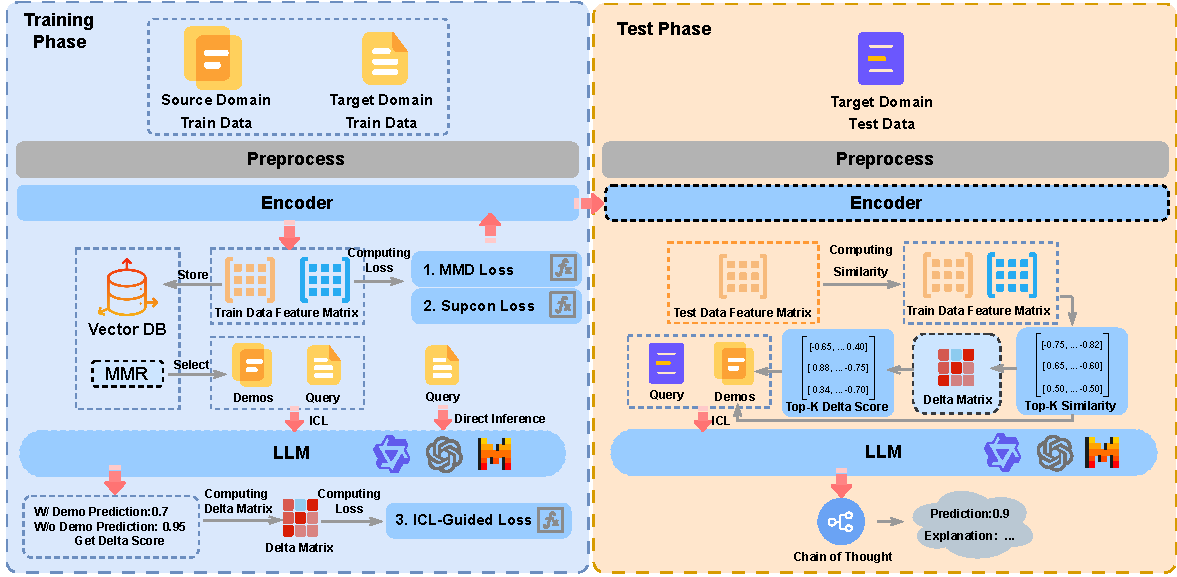
\includegraphics[width=1\textwidth]{Figures/new_overall_framework of LogICL.pdf}
\caption{Overall framework of LogICL.}
\label{fig:logicl_framework}
\end{figure*}

\subsection{Overview}
As illustrated in Figure~\ref{fig:logicl_framework}, LogICL is a framework designed to distill the reasoning capabilities of LLMs into a log sequence encoder for effective cross-domain anomaly detection. The workflow operates in two phases: training and inference(test). During the training phase (left panel), we first construct a sparse delta matrix by evaluating the zero-shot and one-shot performance of an LLM using demonstrations selected via Maximal Marginal Relevance (MMR)~\cite{gretton2012kernel}. This matrix systematically quantifies the directional utility of training samples, providing a robust supervision signal that guides the encoder optimization through a novel ICL-Guided Loss. To ensure comprehensive representation learning, the encoder is jointly optimized using a multi-objective function that integrates the ICL-Guided Loss with Maximum Mean Discrepancy (MMD) for domain alignment and Supervised Contrastive (SupCon) loss for anomaly discrimination. In the inference phase (right panel), LogICL leverages this optimized encoder to retrieve demonstrations based on a hybrid metric of semantic similarity and learned delta utility. These high-quality demonstrations are then fed into the LLM to perform interpretable, Chain-of-Thought (CoT) enhanced anomaly detection on target domain data.

\subsection{Pre-processing}

Traditional log analysis employs parsers (e.g., Drain~\cite{he2017drain}) to split raw log messages into constant \textit{event templates} and dynamic \textit{parameters}, as illustrated in Fig.~\ref{workflow_log_anomaly_detection}. However, this parsing process introduces inherent limitations. First, parsing algorithms may misidentify variable parameters as template tokens. This error generates fragmented templates for logs belonging to the same event category, artificially introducing ``unseen formats'' that inject noise into downstream detection tasks~\cite{chen2021neurallog, jiang2024large, jiang2024lilac, le2023log}. Second, discarding dynamic parameters results in the loss of semantic information that is valuable for detection accuracy. Recent studies indicate that Transformer-based models can achieve robust performance directly on raw log text without explicit parsing~\cite{guan2024logllm, chen2021neurallog}.

Consequently, we adopt a \textbf{parser-free strategy}. We utilize regular expressions for basic preprocessing, which avoids parsing-induced noise while preserving raw parameter details (e.g., IP addresses, \textit{block\_id}). Crucially, retaining these parameters enables the downstream LLM to leverage the full semantic context during inference, thereby enhancing detection accuracy and providing interpretable diagnostics that help operation experts narrow the scope of anomaly localization.

% While traditional methods utilize parsers (e.g., Drain~\cite{he2017drain}) to abstract dynamic parameters into constant tokens, this approach often discards semantic context critical for anomaly localization and generalizes poorly to unseen formats~\cite{chen2021neurallog}. Conversely, LLMs leverage such parameter information for deeper contextual reasoning. Corroborating findings that lightweight preprocessing yields comparable performance to complex parsing for LLM-based tasks~\cite{guan2024logllm}, we adopt a parser-free strategy. We employ minimal regular expressions for noise filtering and normalization, preserving raw semantic content to maximize the reasoning and interpretability of the downstream LLM.

\subsection{Log Sequences Representation Learning}

Following preprocessing, raw log messages are grouped into sequences to capture system execution flows. This is achieved via two strategies: session-based partitioning, which aggregates messages by identifiers (e.g., \textit{block\_id} in HDFS), and window-based partitioning (fixed or sliding) for continuous streams. This structuring is critical as it enables the model to detect anomalies based on sequential dependencies and behavioral patterns, rather than analyzing isolated log entries.

Let a log sequence be denoted as $s=\{ m_1, m_2, \dots, m_L \}$, where $s$ is a sequence of log messages $m_i$, and $L$ is the sequence length. A training dataset of sequences is defined as $\mathcal{D}_{\text{train}} = \{ s_1, s_2, \dots, s_N \}, s_i \in d_s$, where $N$ is the number of sequences in the training dataset. Each log sequence $s_i$ is encoded into a fixed-dimensional embedding vector via the encoder $f_{e}$:
\begin{equation}
\begin{aligned}
v_i &= f_e(s_i) \in \mathbb{R}^d, \quad i = 1, \dots, N,
\end{aligned}
\label{eq:sentencebert}
\end{equation}
% \[
%   v_i = f_\theta(S_i) \in \mathbb{R}^d, \quad i = 1, \dots, N,
% \] 
where $v_i$ denotes the embedding vector of sequence $s_i$ and $d$ is the embedding dimension (i.e., the number of features representing each sequence).

Collectively, the set of embeddings for the training dataset is
\begin{equation}
\begin{aligned}
\mathcal{E} = \{ v_1, v_2, \dots, v_N \} \subset \mathbb{R}^d,
\end{aligned}
\label{eq:feature vector}
\end{equation}
where $\mathcal{E}$ represents the embedding space of all training sequences.

In the context of cross-domain log anomaly detection, the feature extraction stage is critical for effective transfer learning. Ideally, the encoder should generate embeddings that are domain-invariant, improving downstream performance by suppressing irrelevant system-specific variations through domain alignment techniques. However, applying such alignment aggressively can lead to negative transfer. Since distinct systems manifest anomalies through unique semantic keywords—for instance, \textit{block lost} is a critical fault indicator in HDFS, whereas \textit{file system full} plays a similar role in BGL—excessive alignment risks treating these discriminative semantics as domain noise and erasing them. Consequently, a robust representation learning framework must strike a balance: effectively bridging the domain gap while preserving the semantic discriminability of system-specific anomalies.

\subsection{Training Phase}

The training phase of LogICL is composed of two primary stages. First, we construct a delta matrix via ICL on the training set. This matrix quantifies the extent to which a specific demonstration  log sequence contributes to the correct inference of a query sequence. 
Second, we optimize the log sequence encoder using a Multi-Objective Loss Function that integrates ICL-Guided Loss.

\subsubsection{Construction of Delta Matrix}
We construct a delta matrix to systematically quantify the extent to which a specific training sample, acting as a demonstration, enhances the inference accuracy of a target query sequence. Let $\mathcal{S}_{train}=\{s_1,\dots,s_N\}$ denote the training set, where each sequence $s_q$ serves as both a potential query and a demonstration candidate. The construction process involves two steps: demonstrations selection via MMR and influence quantification via delta scores.

\paragraph{Demonstrations Selection}
Exhaustively computing delta scores for all pairwise combinations in the training set $\mathcal{S}_{train}$ entails performing LLM inference $O(N^2)$ times, which is computationally prohibitive. To circumvent this overhead, we prune the search space for each query sequence $s_q$ (with embedding $\mathbf{q}$) by retrieving a dedicated \textit{demonstration set} $\mathcal{D}_q$ of size $k$. Instead of relying solely on cosine similarity—which often yields redundant samples—we employ the MMR algorithm to balance semantic \textbf{relevance} with \textbf{diversity}~\cite{carbonell1998use}.

Formally, we iteratively construct $\mathcal{D}_q$ by selecting samples from the available training pool. Let $S$ denote the subset of demonstrations already selected in previous iterations (initially $S = \varnothing$). In each step, MMR identifies a sample $s^*$ (with embedding $\mathbf{d}^*$) that maximizes the marginal relevance objective:
\begin{equation}
\begin{aligned}
s^* 
&= \operatorname*{arg\,max}_{s_j \in \mathcal{S}_{train} \setminus (S \cup \{s_q\})}
\Big[
\lambda \cdot \text{sim}(\mathbf{q}, \mathbf{d}_j) \\
&\quad - (1 - \lambda) \cdot 
\max_{s_k \in S} \text{sim}(\mathbf{d}_j, \mathbf{d}_k)
\Big]
\end{aligned}
\label{eq:mmr}
\end{equation}
where $\mathbf{d}_j$ and $\mathbf{d}_k$ represent the embeddings of a potential demonstration $s_j$ and an already selected sample $s_k$, respectively. The chosen sample $s^*$ is then added to $S$ until $|S|=k$, at which point $\mathcal{D}_q \leftarrow S$. This procedure ensures that the final demonstration set $\mathcal{D}_q$ covers a broad spectrum of informative cross-domain patterns.

\paragraph{Computation of Delta Scores}
After retrieving the demonstration set $\mathcal{D}_q$ for each query $s_q$, we systematically quantify the contribution of each demonstration $s_d \in \mathcal{D}_q$. We define the delta score, $\delta(s_q, s_d)$, as the reduction in absolute prediction error achieved by conditioning the inference on $s_d$.

Let $l(s_q) \in \{0,1\}$ denote the ground truth label. We define the prediction error in the zero-shot setting as $e_{\text{zero}}(s_q) = |p_0(s_q) - l(s_q)|$, and in the one-shot setting as $e_{\text{one}}(s_q, s_d) = |p_1(s_q \mid s_d) - l(s_q)|$, where $p_0$ and $p_1$ represent the anomaly probabilities predicted by the LLM in the absence and presence of the demonstration $s_d$, respectively. The delta score is formulated as:
\begin{equation}
\label{eq:delta}
\delta(s_q, s_d) = e_{\text{zero}}(s_q) - e_{\text{one}}(s_q, s_d)
\end{equation}
A positive $\delta$ indicates that $s_d$ provides informative context that aligns the prediction with the true label, whereas a negative value suggests the introduction of noise.

Finally, we aggregate these scores into a sparse matrix $\mathbf{M}_\delta \in \mathbb{R}^{N \times N}$. The entry corresponding to query $s_q$ and demonstration $s_d$ is defined as:
\begin{equation}
(\mathbf{M}_\delta)_{qd} = 
\begin{cases} 
\delta(s_q, s_d) & \text{if } s_d \in \mathcal{D}_q \\
0 & \text{otherwise}
\end{cases}
\end{equation}
This selective computation restricts the complexity to $O(N \cdot k)$, effectively filtering out irrelevant pairs while providing a robust supervision signal for the subsequent encoder optimization.

\subsubsection{Multi-Objective Loss Function}

% We design a multi-objective loss function to jointly optimize the encoder for domain alignment, discriminative representation learning, and ICL-based knowledge distillation. 

We design a multi-objective loss function to jointly optimize the encoder, which comprises three components: (1) Domain Alignment Loss, (2) Task-Specific Loss and (3) ICL-Guided Loss. 

\paragraph{Domain Alignment Loss} To mitigate the discrepancy between source and target domains, we introduce a Domain Alignment Loss that enforces similarity between their latent feature distributions. The objective is to learn domain-invariant representations, such that feature embeddings from the source and target domains become indistinguishable in a shared latent space, thereby facilitating more effective cross-domain demonstration selection during ICL inference. This alignment is realized by minimizing the distributional discrepancy between the two domains through the Maximum Mean Discrepancy (MMD) criterion \cite{gretton2012kernel}. Specifically, MMD quantifies the distance between the feature embeddings of log sequences from the source and target domains in a Reproducing Kernel Hilbert Space (RKHS) \cite{sriperumbudur2010hilbert}. By reducing this distance, the encoder learns to produce domain-invariant embeddings that capture task-relevant semantics while suppressing domain-specific biases, thus promoting more consistent and transferable reasoning across domains.

\begin{equation}
\scalebox{0.9}{$
\begin{aligned}
L_{\text{MMD}} &= 
\left\| 
\frac{1}{N_h} \sum_{i=1}^{N_h} \phi(\text{Encoder}(s_{h_i})) 
- \frac{1}{N_b} \sum_{j=1}^{N_b} \phi(\text{Encoder}(s_{b_j})) 
\right\|_H
\end{aligned}
$}
\end{equation}

  % \[
  % L_{\text{MMD}} = \left\| \frac{1}{N_h} \sum_{i=1}^{N_h} \phi(\text{Encoder}(\text{s}_{h_i})) - \frac{1}{N_b} \sum_{j=1}^{N_b} \phi(\text{Encoder}(\text{s}_{b_j})) \right\|_H
  % \]
  where $\phi$ is a Gaussian kernel, $N_h$ and $N_b$ are batch sizes for each domain, and $H$ is the RKHS. This ensures embeddings are domain-consistent, facilitating source-to-target transfer in few-shot settings.

\paragraph{Task-Specific Loss} To enhance the discriminative capacity of the encoder, We employ a Supervised Contrastive Loss that encourages positive log sequence pairs (with the same label) to have closer embeddings in the representation space, while increasing the distance between negative pairs (log sequences with different labels) \cite{khosla2020supervised}. By leveraging label information, this loss explicitly strengthens intra-class cohesion and inter-class separation, leading to more structured and semantically consistent feature representations. Such discriminative embeddings provide a stronger foundation for downstream anomaly detection task:

\begin{equation}
\scalebox{0.78}{$
\begin{aligned}
L_{\text{SupCon}} &= \frac{1}{B} \sum_{b=1}^B \sum_{i \in I_b} 
\frac{-1}{|P(i)|} \sum_{p \in P(i)} 
\log \left( 
\frac{\exp(s_{i,p} / \tau) + \epsilon}{
\sum_{a \in A(i)} \exp(s_{i,a} / \tau) + \epsilon} 
\right)
\end{aligned}
$}
\end{equation}

where $B$ denotes the batch size, $v_i = f_\theta(s_i) \in \mathbb{R}^d$ is the embedding vector of log sequence $s_i$ encoded via the encoder $f_\theta$, $P(i)$ denotes the set of positive log sequences sharing the same label as $s_i$, $A(i)$ is the set of all log sequences in the batch, $s_{i,p} = \text{sim}(v_i, v_p)$ for $v_p \in P(i)$ forming a positive pair with $v_i$, and $s_{i,a} = \text{sim}(v_i, v_a)$ for $v_a \in A(i)$.

\paragraph{ICL-Guided Loss} We introduce an ICL-Guided Loss based on the sparse delta matrix $\mathbf{M}_\delta$ to align the log sequence encoder with the LLM's inference behavior. This objective optimizes the embedding space to ensure retrieval selects demonstrations that improve prediction performance. As illustrated in Figure~\ref{fig:loss_opt}, after constructing delta matrix, the loss explicitly regulates vector distances based on ICL utility: the model pulls queries closer to demonstrations with positive delta scores, and pushes away those with negative scores. By utilizing sparse delta matrix $\mathbf{M}_\delta$, the optimization processes only validated, informative pairs, ensuring efficient knowledge transfer without introducing noise from irrelevant sample combinations. The loss function consists of the following two components:

\begin{figure}[htbp]
\centerline{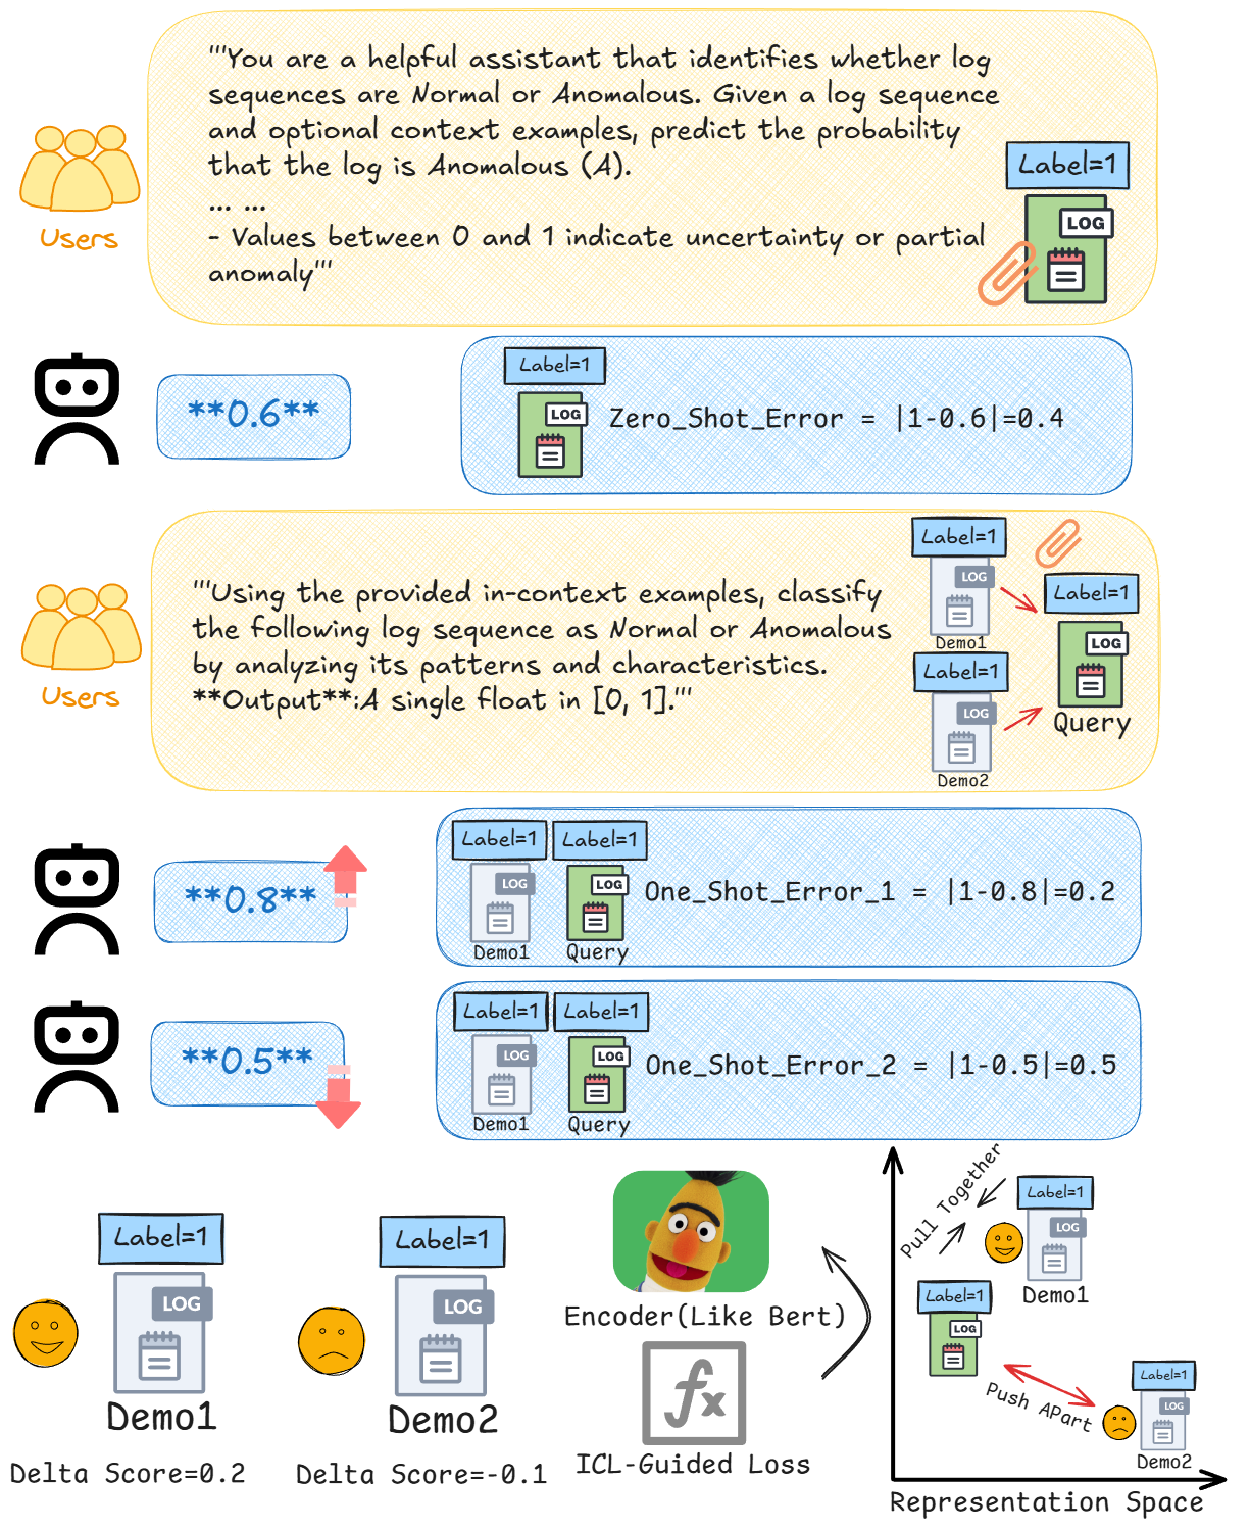
\includegraphics[scale=0.4]{Figures/new_icl_guided_loss.pdf}}
\caption{Illustration of ICL-Guided Loss.}
\label{fig:loss_opt}
\end{figure}

% We utilize the sparse delta matrix  $\mathbf{M}_\delta$ to optimize encoder, encouraging positive pairs to be closer and negative pairs to be farther apart in the representation space, while avoiding undue penalization. 
\begin{itemize}
\item The loss function for positive pairs ($D^+$) is formulated to increase the similarity between sample pairs to improve ICL inference accuracy.
% We use the Delta matrix to optimize for ICL, reinforcing positive pairs and weakening negative ones without excessive penalty:
%   For positive pairs ($D^+$):
    % Defining the compact Delta+ loss formula
    \begin{equation}
    \label{eq: pos_delta_loss}
    \begin{aligned}
    L_{\text{Delta+}} &= -\sum_{(i,j) \in D^+} \delta(s_q, s_d) \cdot \log \left( \frac{s_{i,j}}{\tau} \right)
    \end{aligned}
    \end{equation}
    
    % Integrated and compact explanation
    where $D^+$ denotes the set of positive log sequence pairs, $\delta(s_q, s_d)$ is the delta score between query log sequence $s_q$ and demonstration $s_d$, and $s_{i,j} = \text{sim}(v_i, v_j)$ denotes the cosine similarity between the embeddings of $s_i$ and $s_j$, with $\tau$ as the temperature scaling factor.

\item The loss function for negative pairs ($D^-$) is formulated to reduce the embedding similarity between them.
  % Defining the compact Delta- loss formula
    \begin{equation}
    \label{eq: neg_delta_loss}
    \scalebox{0.93}{$
    \begin{aligned}
    L_{\text{Delta-}} &= \sum_{(i,j) \in D^-} \max(0, |\delta(s_q, s_d)| - \theta) \cdot (1 - s_{i,j})
    \end{aligned}
    $}
    \end{equation}
    
  \end{itemize}
The complete loss function is formulated as follows:
    \begin{equation}
    \label{eq:delta_loss}
    \begin{aligned}
    L_{\text{Delta}} &= L_{\text{Delta+}} + \lambda_{\text{Delta-}} \cdot L_{\text{Delta-}}
    \end{aligned}
    \end{equation}

where $\lambda_{\text{Delta-}}$ handles negative deltas by ignoring small interferences, balancing ICL guidance with domain consistency. Combining the above three types of loss functions, the overall Multi-Objective Loss Function $L_{\text{Multi}}$ is formulated as follows:
\begin{equation}
\label{eq:total_loss}
\scalebox{0.95}{$
\begin{aligned}
L_{\text{Multi}} &= \lambda_{\text{MMD}} \cdot L_{\text{MMD}} 
+ \lambda_{\text{SupCon}} \cdot L_{\text{SupCon}} 
+ \lambda_{\text{Delta}} \cdot L_{\text{Delta}}
\end{aligned}
$}
\end{equation}
where $\lambda_{\text{MMD}}$, $\lambda_{\text{SupCon}}$, and $\lambda_{\text{Delta}}$ are hyperparameters controlling the relative importance of the domain alignment, task-specific, and ICL-Guided losses, respectively.

\subsection{Test Phase}

During inference, we employ a \textit{Dual-Source Retrieval Strategy} to construct optimal in-context demonstrations. For a given test log $s_t$, encoded as \( v_t = f'_{\text{encoder}}(s_t) \), the selection process proceeds in two stages to balance surface lexical similarity and latent semantic equivalence:

\subsubsection{Similarity-based Anchoring}
We first retrieve the \textit{top-i} nearest neighbors from the training set $\mathcal{D}_{train}$ based on cosine similarity to $s_t$. These samples form the similarity-based anchor set $\mathcal{C}_{sim}$:
\begin{equation}
\label{eq:anchor_sim}
\setlength{\abovedisplayskip}{3pt}
\setlength{\belowdisplayskip}{3pt}
\mathcal{C}_{sim} = \mathop{top\textit{-}i}_{s_j \in \mathcal{D}_{train}} \left( \frac{v_t \cdot v_j}{\|v_t\| \|v_j\|} \right)
\end{equation}

\subsubsection{Delta-guided Expansion}
We leverage the retrieved anchors in $\mathcal{C}_{sim}$ to query the pre-computed delta matrix. The underlying assumption is that optimal demonstrations for the anchors are likely effective for the test sample due to their high similarity. Specifically, we select the \textit{top-j} training samples that yielded the highest delta scores for the anchors in $\mathcal{C}_{sim}$. We aggregate these pre-computed scores and select the \textit{top-j} samples to form the expansion set $\mathcal{C}_{delta}$:

\begin{equation}
\setlength{\abovedisplayskip}{3pt}
\setlength{\belowdisplayskip}{3pt}
\mathcal{C}_{delta} = \mathop{top\textit{-}j}_{s_n \in \mathcal{D}_{train}} \left( \sum_{s_m \in \mathcal{C}_{sim}} \delta_{m,n} \right)
\end{equation}

\noindent where $\delta_{m,n}$ represents the pre-computed delta score of using $s_n$ as a demonstration for anchor $s_m$. Finally, the LLM performs anomaly detection using the combined context $\mathcal{C}_{final} = \mathcal{C}_{sim} \cup \mathcal{C}_{delta}$.

\subsubsection{In-context and CoT Prediction}
The set $\mathcal{C}_{final} = \{s_{1}, s_{2}, \dots, s_{k}\}$ is selected to assist the LLM in performing inference on the test log $s_t$, where $\{y_{1}, y_{2}, \dots, y_{k}\}$ denote the corresponding labels.
\begin{equation}
\mathcal{P}_t = \{(s_{1}, y_{1}), (s_{2}, y_{2}), \dots, (s_{k}, y_{k}), s_t\}.
\end{equation}

The prompt $\mathcal{P}_t$ is then provided to the LLM to estimate the anomaly probability of the test log $s_t$:
\begin{equation}
p_t = \textit{LLM}(\mathcal{P}_t),
\end{equation}
where \(p_t \in [0,1]\) denotes the probability that \(s_t\) is anomalous.  
When CoT reasoning is enabled, the model provides a step-by-step diagnostic explanation before outputting \(p_t\).

\section{EVALUATION}

\subsection{Experimental Design}
\subsubsection{Datasets}
We evaluate our method on four public log benchmarks: HDFS, BGL, Thunderbird, and Liberty. These datasets encompass diverse system architectures and data distributions, providing a comprehensive testbed to evaluate the model's generalization capabilities. \cite{oliner2007supercomputers}.
\begin{itemize}
    \item \textbf{Distributed File System Logs.} Represented by HDFS, this dataset is collected from 200 Amazon EC2 nodes and contains 11.18 million messages with a 2.93\% anomaly ratio \cite{xu2009detecting}.
    
    \item \textbf{Supercomputing System Logs.} This category includes BGL, Thunderbird, and Liberty, which are derived from high-performance computing environments but exhibit distinct alert characteristics. 
    BGL is dominated by hardware alerts (98.04\%) with a 7.34\% anomaly ratio. 
    In contrast, Thunderbird and Liberty primarily feature software-related alerts. Notably, Liberty presents a challenge of extreme imbalance with scarce anomalies, whereas Thunderbird contains a complex mix of uncertainty alerts \cite{oliner2007supercomputers}.
\end{itemize}

\subsubsection{Data Preprocessing and Sampling}
We adopt distinct log grouping strategies based on the dataset structure. For HDFS, log messages are grouped by their unique \textit{block\_id}. For supercomputing datasets (BGL, Thunderbird, and Liberty), we employ fixed sliding windows (non-overlapping), setting the window size to 40 for BGL and Thunderbird, and 30 for Liberty. To prevent data leakage, we partition the training and testing sets strictly in chronological order. The resulting training dataset consists of 50,000 source domain sequences and only 5,000 target domain sequences.

\begin{table}[htbp]
    \centering
    \small % 保持小号字体
    \setlength{\tabcolsep}{6pt} % 保持列间距
    
    % 保持标题样式为小型大写 + 无句号
    \caption{\textsc{Details of the datasets}}
    \label{tab:dataset_details}
    
    % 修改处：将第一个 l 改为 c，使 Dataset 列居中
    \begin{tabular}{@{} c c c c @{}}
        \toprule
        \textbf{Dataset} & \textbf{Log Messages} & \textbf{Log Seq} & \textbf{Anomaly Log Seq} \\
        \midrule
        HDFS & 11,175,629 & 575,061 & 16,838 \\
        BGL & 4,713,520 & 117,838 & 24,697 \\
        Thunderbird & 20,000,000 & 500,000 & 24,697 \\
        Liberty & 5,000,000 & 166,667 & 110,427 \\ 
        \bottomrule
    \end{tabular}
\end{table}

% \begin{table}[h]
%     \centering
%     % 这一行用于增加行高，使内容在垂直方向上看起来更居中、更舒展
%     \renewcommand{\arraystretch}{1.5} 
%     \caption{Detail of the datasets}
%     % 将 lccc 改为 cccc，实现所有列水平居中
%     \begin{tabular}{cccc} 
%         \toprule
%         \textbf{Datasets} & \textbf{Log Messages} & \textbf{Log Seq} & \textbf{Anomaly Log Seq} \\
%         \midrule
%         HDFS & 11,175,629 & 575,061 & 16,838 \\
%         BGL & 4,713,520 & 117,838 & 24,697 \\
%         Thunderbird & 20,000,000 & 500,000 & 24,697 \\
%         Liberty & 5,000,000 & 166,667 & 110,427 \\ 
%         \bottomrule
%     \end{tabular}
% \end{table}

% \paragraph{Cross-domain Transfer Settings}
% To comprehensively evaluate the cross-domain generalization capability of the proposed model, we design two types of transfer experiments: \textbf{few-shot} and \textbf{zero-shot} settings. 
% In the \textbf{few-shot transfer} scenario, limited labeled samples from the target domain are available during training, allowing the model to adapt its representation to new domains with minimal supervision. 
% We construct four few-shot configurations: \textit{HDFS + BGL $\rightarrow$ BGL}, \textit{HDFS + Thunderbird $\rightarrow$ Thunderbird}, \textit{BGL + Liberty $\rightarrow$ Liberty}, and \textit{BGL + Thunderbird $\rightarrow$ Thunderbird}. 
% To further assess the model’s cross-domain generalization without any target-domain exposure, we conduct \textbf{zero-shot transfer} experiments, including \textit{HDFS + BGL $\rightarrow$ Liberty} and \textit{Thunderbird + BGL $\rightarrow$ Liberty}. 
% This dual-setting design enables a comprehensive analysis of how the model performs under different levels of domain supervision.

% \paragraph{Cross-domain Transfer Settings}
% To evaluate the generalization capability of LogICL, we conduct experiments on four datasets: HDFS, BGL, Thunderbird (TB), and Liberty.
% We design two transfer scenarios:
% (1) \textbf{Few-Shot Transfer}, where the model adapts using limited labeled samples (e.g., $k=8$) from the target domain;
% and (2) \textbf{Zero-Shot Transfer}, where the target domain remains unseen during the setup. This design assesses performance under varying levels of domain supervision.

\subsubsection{Cross-domain Transfer Settings}To evaluate the generalization capability of LogICL across HDFS, BGL, Thunderbird (TB), and Liberty, we design two settings with strictly defined data splits: (1) few-shot transfer: Simulating limited target supervision, the training set combines 50,000 source samples with 5,000 target samples. As shown in Table \ref{tab:few_shot_results}  (e.g., Liberty-BGL). During inference, $k=8$ demonstrations are retrieved specifically from the training set to predict the test data. (2) zero-shot transfer: To assess robustness on unseen domains, the training set combines 50,000 primary source domain samples with 5,000 auxiliary source domain samples. As shown in Table \ref{tab:zero_shot_results} (e.g., the BGL-Liberty-TB), the model retrieves $k=8$ demonstrations from primary source samples (BGL) and auxiliary source domain samples (Liberty) to predict unseen target domain samples (TB).


\subsubsection{Baselines}
To comprehensively evaluate the effectiveness of LogICL, we benchmark it against nine representative methods across three paradigms:
\begin{itemize}
    \item \textbf{Deep Learning-based Approaches:} We include LogRobust \cite{zhang2019robust} as a standard supervised baseline. This method transforms distinct log events into semantic vectors and employs a Long Short-Term Memory (LSTM) network to capture temporal patterns and contextual semantics, enabling stable anomaly detection across variable log data. 
    \item \textbf{Cross-System Approach:} For cross-system scenarios, we adopt LogTransfer\cite{chen2020logtransfer}, LogTAD\cite{han2021unsupervised} and MetaLog\cite{zhang2024metalog}, which utilize transfer learning and meta-learning techniques to adapt to target domains.
    \item \textbf{LLM-based Approaches:} This category assesses the effectiveness of LLM-based strategies, comprising both fine-tuned and parameter-frozen approaches. LogLLM first encodes log sequences into feature vectors and then performs efficient supervised fine-tuning of the LLM for anomaly detection. Among the frozen models, LogPrompt utilizes zero-shot prompting, relying solely on the LLM's intrinsic knowledge. LogRAG \cite{zhang2024lograg} is a hybrid unsupervised method combining a DeepSVDD classifier with Retrieval-Augmented Generation (RAG) technology. Furthermore, Random-ICL and $k$NN-ICL represent standard ICL baselines from the general NLP domain for text classification \cite{qin2024context, peng2024revisiting}. We include these two to specifically evaluate whether generic ICL strategies suffice for this specialized task; Random-ICL establishes a lower performance bound by selecting demonstrations randomly, whereas $k$NN-ICL selects examples based on $k$-nearest neighbor matching for semantic similarity.
\end{itemize}

% \paragraph{Evaluation Metrics} 
% To balance the trade-off between precision ($P$) and recall ($R$), we adopt the F1-Score ($F_1 = 2PR/(P+R)$) as the primary evaluation metric. Here, $P = TP/(TP+FP)$ and $R = TP/(TP+FN)$, where $TP$, $FP$, and $FN$ denote true positives, false positives, and false negatives, respectively. Consistent with standard practices, we apply a classification threshold of 0.5 across all models to determine anomaly labels.
% \paragraph{Evaluation Metrics}
\subsubsection{Evaluation Metrics}
We choose Precision, Recall, and F1-Score as the evaluation measurements, with the definitions of $\mathit{Precision} = \frac{\mathit{TP}}{\mathit{TP}+\mathit{FP}}$, $\mathit{Recall} = \frac{\mathit{TP}}{\mathit{TP}+\mathit{FN}}$, and $\mathit{F1} = \frac{2 \cdot \mathit{Precision} \cdot \mathit{Recall}}{\mathit{Precision} + \mathit{Recall}}$. Here, $\mathit{TP}$, $\mathit{FP}$, and $\mathit{FN}$ denote the number of true positives, false positives, and false negatives, respectively. 

\subsubsection{Implementation Details}
We implement our framework in PyTorch with Python 3.11, accelerated by two NVIDIA H200 GPUs (141~GB). We employ Sentence-BERT as the backbone encoder. It maps log sequence to a 384-dimensional dense vector space, while Qwen-14B serves as the core LLM, deployed via vLLM. In the training phase, we iterate through each training sample as a query and employ MMR to retrieve 128 candidates for constructing the delta matrix. In the test phase, we retrieve 8 demonstrations for each test query to perform inference. The weighting coefficients for the multi-objective loss are empirically set to $\lambda_{\text{MMD}} = 0.1$, $\lambda_{\text{SupCon}} = 1.0$, and $\lambda_{\text{Delta}} = 1.0$. Consistent with standard practices, we apply a classification threshold of 0.5 to determine anomaly labels. Our code is open-sourced in \url{https://zenodo.org/records/17482762}

\begin{table*}[htbp]
\centering
\caption{\textsc{Evaluation under Cross-Domain Few-Shot Transfer Setting (Precision, Recall, F1-Score).}}
\label{tab:few_shot_results}
\renewcommand{\arraystretch}{1.25} % 适当增加行高
\setlength{\tabcolsep}{4pt} % 微调列间距
\small
\resizebox{\textwidth}{!}{%
\begin{tabular}{c c ccc ccc ccc ccc}
\toprule
% 表头第一行
\multirow{2}{*}[-2pt]{\textbf{Method}} & \multirow{2}{*}[-2pt]{\textbf{Type}} 
& \multicolumn{3}{c}{\textbf{Liberty-BGL}}
& \multicolumn{3}{c}{\textbf{BGL-TB}}
& \multicolumn{3}{c}{\textbf{BGL-Liberty}}
& \multicolumn{3}{c}{\textbf{TB-Liberty}} \\

\cmidrule(lr){3-5} \cmidrule(lr){6-8} \cmidrule(lr){9-11} \cmidrule(lr){12-14}

% 表头第二行
& & P(\%) & R(\%) & F1(\%) 
& P(\%) & R(\%) & F1(\%) 
& P(\%) & R(\%) & F1(\%) 
& P(\%) & R(\%) & F1(\%) \\

\midrule
% --- Traditional / Supervised Methods ---
LogRobust & Supervised
& 39.01 & 87.06 & 53.88 
& 4.78 & 0.01 & 0.03
& 6.99 & 0.12 & 0.23
& 54.66 & 2.53 & 4.83 \\ 

LogTransfer & Supervised Cross-System
& 0.00 & 0.00 & 0.00
& 33.84 & 100.00 & 50.57
& 0.00 & 0.00 & 0.00
& 0.00 & 0.00 & 0.00 \\

LogTAD & Unsupervised Cross-System
& 62.60 & 58.33 & 59.91
& 60.77 & 61.10 & 60.87
& 86.49 & 66.24 & 66.95
& 84.41 & 67.50 & 68.63 \\

MetaLog & Supervised Cross-System
& 65.78 & 59.09 & 62.26
& 47.03 & 99.87 & 63.94
& 35.02 & 54.33 & 42.59
& 80.98 & 89.58 & 85.06 \\

\midrule % 分隔线：传统方法 vs LLM方法

% --- LLM-based Methods ---
LogLLM & LLM-based (fine-tune)
& 40.55 & 11.13 & 17.47
& 70.87 & 37.94 & 49.43
& 59.09 & 99.91 & 74.26
& - & - & - \\

LogPrompt & LLM-based (frozen)
& 39.35 & 76.61 & 52.00
& 51.12 & 70.65 & 59.32
& 66.62 & 47.30 & 55.32
& - & - & - \\

LogRAG & Unsupervised \& LLM (frozen)
& 91.00 & 98.56 & 29.13
& 44.66 & 100.00 & 61.74
& 88.40 & 100.00 & \textbf{93.84}
& - & - & - \\

Random-ICL & LLM-based (frozen)
& 29.96 & 100.00 & 34.65 
& 30.82 & 100.00 & 47.12 
& 66.26 & 100.00 & 79.71 
& 65.53 & 96.44 & 78.04 \\

$k$NN-ICL & LLM-based (frozen)
& 29.31 & 31.28 & 30.26 
& 40.13 & 37.85 & 38.95 
& 33.80 & 6.62 & 11.07 
& 90.58 & 53.77 & 67.48 \\

% --- 修改处：在这里加了 midrule，把 kNN-ICL 和 LogICL 隔开 ---
\midrule 

% --- Ours ---
\textbf{LogICL (Ours)} & \textbf{LLM-based (frozen)}
& 70.29 & 78.21 & \textbf{74.04}
& 91.16 & 87.54 & \textbf{89.32}
& 74.44 & 85.43 & 79.56
& 81.83 & 88.87 & \textbf{85.20} \\

\bottomrule
\end{tabular}%
}
\end{table*}

% \begin{table*}[htbp]
% \centering
% \caption{Evaluation under Cross-Domain Few-Shot Transfer Setting (Precision, Recall, F1-Score).}
% \label{tab:few_shot_results}
% \renewcommand{\arraystretch}{1.3}
% \small
% \resizebox{\textwidth}{!}{%
% \begin{tabular}{c c  |c c c  |c c c  |c c c  |c c c}
% \toprule
% \centering\textbf{Method} & \centering\textbf{Type} 
% & \multicolumn{3}{c|}{\textbf{Liberty-BGL}}
% & \multicolumn{3}{c|}{\textbf{BGL-TB}}
% & \multicolumn{3}{c|}{\textbf{BGL-Liberty}}
% & \multicolumn{3}{c}{\textbf{TB-Liberty}} \\

% \cmidrule(lr){3-5}
% \cmidrule(lr){6-8}
% \cmidrule(lr){9-11}
% \cmidrule(lr){12-14}

% & & P(\%) & R(\%) & F1(\%) 
% & P(\%) & R(\%) & F1(\%) 
% & P(\%) & R(\%) & F1(\%) 
% & P(\%) & R(\%) & F1(\%) \\

% \midrule
% LogRobust & Supervised
% & 39.01 & 87.06 & 53.88 
% & 4.78 & 0.01 & 0.03
% & 6.99 & 0.12 & 0.23
% & 54.66 & 2.53 & 4.83 \\ 

% LogTransfer & Supervised Cross-System
% & 0 & 0 & 0
% & 33.84 & 100 & 50.57
% & 0 & 0 & 0
% & 0 & 0 & 0 \\

% LogTAD & Unsupervised Cross-System
% & 62.60 & 58.33 & 59.91
% & 60.77 & 61.10 & 60.87
% & 86.49 & 66.24 & 66.95
% & 84.41 & 67.50 & 68.63 \\

% MetaLog & Supervised Cross-System
% & 65.78 & 59.09 & 62.26
% & 47.03 & 99.87 & 63.94
% & 35.02 & 54.33 & 42.59
% & 80.98 & 89.58 & 85.06 \\

% LogLLM & LLM-based(fine-tune)
% & 40.55 & 11.13 & 17.47
% & 70.87 & 37.94 & 49.43
% & 59.09 & 99.91 & 74.26
% & - & - & - \\

% LogPrompt & LLM-based(parameters frozen)
% & 39.35 & 76.61 & 52.00
% & 51.12 & 70.65 & 59.32
% & 66.62 & 47.30 & 55.32
% & - & - & - \\

% LogRAG & Unsupervised \& LLM-based(parameters frozen)
% & 91.00 & 98.56 & 29.13
% & 44.66 & 100 & 61.74
% & 88.40 & 100 & \textbf{93.84}
% & - & - & - \\

% Random-ICL & LLM-based(parameters frozen)
% & 29.96& 100& 34.65& 
% 30.82& 100& 47.12& 
% 66.26& 100& 79.71& 
% 65.53& 96.44& 78.04\\

% $knn$-ICL & LLM-based(parameters frozen)
% & 29.31& 31.28& 30.26& 
% 40.13& 37.85& 38.95& 
% 33.8& 6.62& 11.07& 
% 90.58& 53.77& 67.48\\

% \textbf{LogICL (Ours)} & \textbf{LLM-based(parameters frozen)}
% & 70.29 & 78.21 & \textbf{74.04}
% & 91.16 & 87.54 & \textbf{89.32}
% & 74.44 & 85.43 & 79.56
% & 81.83 & 88.87 & \textbf{85.20} \\

% \bottomrule
% \end{tabular}%
% }
% \end{table*}





% \begin{table*}[htbp]
% \centering
% \caption{Evaluation under Cross-Domain Zero-Shot Transfer Setting.}
% \label{tab:zero-shot_results}
% \renewcommand{\arraystretch}{1.3}
% \small
% \resizebox{\textwidth}{!}{%
% \begin{tabular}{c c | c c c | c c c | c c c}
% \toprule
% \centering\textbf{Method} & \centering\textbf{Type} & 
% \multicolumn{3}{c|}{\textbf{BGL}} & 
% \multicolumn{3}{c|}{\textbf{Liberty}} & 
% \multicolumn{3}{c}{\textbf{TB}} \\
% \cmidrule(lr){3-5} \cmidrule(lr){6-8} \cmidrule(lr){9-11}
%  &  & P(\%) & R(\%) & F1(\%) & P(\%) & R(\%) & F1(\%) & P(\%) & R(\%) & F1(\%) \\
% \midrule
% LogRobust & Supervised &  &  &  &  &  &  &  &  &  \\
% NeuralLog & Supervised &  &  &  &  &  &  &  &  &  \\
% LogLLM & Supervised (LLM) &  &  &  &  &  &  &  &  &  \\
% LogTAD & Unsupervised Cross-System &  &  &  &  &  &  &  &  &  \\
% LogSynergy & Supervised Cross-System &  &  &  &  &  &  &  &  &  \\
% LogTransfer & Supervised Cross-System &  &  &  &  &  &  &  &  &  \\
% MetaLog & Supervised Cross-System &  &  &  &  &  &  &  &  &  \\
% \textbf{LogICL (Ours)} & \textbf{Proposed} &  &  &  &  &  &  &  &  &  \\
% \bottomrule
% \end{tabular}%
% }
% \end{table*}


\begin{table*}[htbp]
\centering
\caption{\textsc{Evaluation under Cross-Domain Zero-Shot Transfer Setting (Precision, Recall, F1-Score).}}
\label{tab:zero_shot_results}
\renewcommand{\arraystretch}{1.25} % 保持与表1一致的行高
\setlength{\tabcolsep}{2pt} % 针对17列的密集表格，微调列间距以保持美观
\small
\resizebox{\textwidth}{!}{%
\begin{tabular}{c c ccc ccc ccc ccc ccc}
\toprule
% 表头：垂直居中 + 分组
\multirow{2}{*}[-2pt]{\textbf{Method}} & \multirow{2}{*}[-2pt]{\textbf{Type}} 
& \multicolumn{3}{c}{\textbf{BGL-Liberty-TB}} 
& \multicolumn{3}{c}{\textbf{Liberty-BGL-TB}} 
& \multicolumn{3}{c}{\textbf{TB-Liberty-BGL}} 
& \multicolumn{3}{c}{\textbf{BGL-TB-Liberty}} 
& \multicolumn{3}{c}{\textbf{TB-Liberty-HDFS}} \\

\cmidrule(lr){3-5} \cmidrule(lr){6-8} \cmidrule(lr){9-11} \cmidrule(lr){12-14} \cmidrule(lr){15-17}

& & P(\%) & R(\%) & F1(\%) 
& P(\%) & R(\%) & F1(\%) 
& P(\%) & R(\%) & F1(\%) 
& P(\%) & R(\%) & F1(\%) 
& P(\%) & R(\%) & F1(\%) \\

\midrule
LogRobust & Supervised 
& 57.36 & 91.79 & 70.60 
& 18.07 & 4.59 & 7.32 
& 66.48 & 31.69 & 42.92 
& 79.15 & 5.29 & 9.91 
& 2.43 & 82.50 & 4.73 \\

LogPrompt & LLM-based (frozen)
& 51.12 & 70.65 & 59.32 
& - & - & - 
& 39.35 & 76.61 & \textbf{52.00} 
& 66.62 & 47.30 & 55.32 
& 8.73 & 84.07 & 15.81 \\

MetaLog & Supervised Cross-System 
& 42.10 & 86.23 & 56.58 
& 56.70 & 73.50 & 64.01 
& 29.16 & 23.35 & 25.93 
& 90.72 & 10.02 & 18.04 
& 3.50 & 0.50 & 0.10 \\

\midrule
\textbf{LogICL (Ours)} & \textbf{LLM-based (frozen)} 
& 70.16 & 79.83 & \textbf{74.68} 
& 65.96 & 66.06 & \textbf{66.01} 
& 40.21 & 34.71 & 37.25 
& 82.39 & 69.70 & \textbf{75.52} 
& 72.87 & 22.57 & \textbf{34.68} \\
\bottomrule
\end{tabular}%
}
\end{table*}

% \begin{table*}[htbp]
% \centering
% \caption{Evaluation under Cross-Domain Zero-Shot Transfer Setting (Precision, Recall, F1-Score).}
% \label{tab:zero_shot_results}
% \renewcommand{\arraystretch}{1.3} % 调整行高
% \small 
% % 必须在导言区添加 \usepackage{multirow}
% \resizebox{\textwidth}{!}{%
% \begin{tabular}{c c | c c c | c c c | c c c | c c c | c c c}
% \toprule
% % 使用 multirow 让 Method 和 Type 在垂直方向居中跨越两行
% \multirow{2}{*}{\textbf{Method}} & \multirow{2}{*}{\textbf{Type}} & \multicolumn{3}{c|}{\textbf{BGL-Liberty-TB}} & \multicolumn{3}{c|}{\textbf{Liberty-BGL-TB}} & \multicolumn{3}{c|}{\textbf{TB-Liberty-BGL}} & \multicolumn{3}{c|}{\textbf{BGL-TB-Liberty}} & \multicolumn{3}{c}{\textbf{TB-Liberty-HDFS}} \\
% \cmidrule(lr){3-5} \cmidrule(lr){6-8} \cmidrule(lr){9-11} \cmidrule(lr){12-14} \cmidrule(lr){15-17}
%  &  & P(\%) & R(\%) & F1(\%) & P(\%) & R(\%) & F1(\%) & P(\%) & R(\%) & F1(\%) & P(\%) & R(\%) & F1(\%) & P(\%) & R(\%) & F1(\%) \\
% \midrule
% LogRobust & Supervised & 57.36 & 91.79 & 70.60 & 18.07 & 4.59 & 7.32 & 66.48 & 31.69 & 42.92 & 79.15 & 5.29 & 9.91 & 2.43 & 82.50 & 4.73 \\
% LogPrompt & LLM-based(parameters frozen) & 51.12 & 70.65 & 59.32 & - & - & - & 39.35 & 76.61 & \textbf{52.00} & 66.62 & 47.30 & 55.32 & 8.73 & 84.07 & 15.81 \\
% MetaLog & Supervised Cross-System & 42.10 & 86.23 & 56.58 & 56.70 & 73.50 & 64.01 & 29.16 & 23.35 & 25.93 & 90.72 & 10.02 & 18.04 & 3.50 & 0.5 & 0.10 \\
% \textbf{LogICL (Ours)} & Proposed & 70.16 & 79.83 & \textbf{74.68} & 65.96 & 66.06 & \textbf{66.01} & 40.21 & 34.71 & 37.25 & 82.39 & 69.70 & \textbf{75.52} & 72.87 & 22.57 & \textbf{34.68} \\
% \bottomrule
% \end{tabular}%
% }
% \end{table*}

% We evaluate on HDFS-BGL (structural vs. hardware, 1000 each), HDFS-Thunderbird (scale differences, 1000 HDFS + 2000 Thunderbird), and BGL-Liberty (hardware vs. software, 1000 each). Metrics: accuracy, precision, recall, F1, AUC-ROC. Baselines: vanilla BERT-ICL, SVM, clustering. We emphasize few-shot gains (e.g., 5-10 shots) from source transfer.


\subsection{Evaluation under Cross-Domain Few-Shot Settings}

To comprehensively evaluate the effectiveness of our proposed framework, we compare LogICL with a wide range of baselines. Table~\ref{tab:few_shot_results} presents the comparative results in terms of Precision, Recall, and F1-Score across four cross-domain scenarios.

% \paragraph{Baselines and Experimental Configurations}
\subsubsection{Baselines and Experimental Configurations}
It is important to clarify the specific experimental configurations adopted to ensure a fair and realistic comparison, particularly where they deviate from the original papers:
\begin{itemize}
    \item For LogRobust, we adjusted its original fully supervised setting (using an 8:2 split for training and testing) to align with our cross-domain few-shot setting. It was trained on 50,000 source domain samples and adapted using 5,000 target domain samples.
    \item For LogTransfer and LogTAD, we employ the same source and target domain splits as LogICL. The training and testing sample quantities are kept strictly consistent across all experiments to ensure a fair comparison.
    
    % LogTransfer shows limited effectiveness in the Liberty-BGL, BGL-Liberty, and TB-Liberty scenarios. This is attributed to the data imbalance inherent in the strict chronological split used in our evaluation. While the original LogTransfer implementation requires at least 300 anomaly samples for effective transfer, the 5,000 train from target domain did not meet this threshold. Consequently, the model collapsed to a trivial solution, classifying all instances as benign.
    \item For LogLLM, LogPrompt, and LogRAG, since their original architectures do not inherently support cross-domain transfer mechanisms, we followed their respective intra-domain settings using the 5,000 target domain samples for training. As a result, the experimental setup for TB-Liberty becomes identical to BGL-Liberty (both relying solely on the Liberty target data); thus, we omit redundant results for TB-Liberty (marked as ``-'').
    \item For Random-ICL and $k$NN-ICL, we construct a shared demonstration pool comprising 50,000 labeled source-domain samples and 5,000 labeled target-domain samples. During inference, demonstrations are retrieved from this pool via random sampling or $k$-nearest neighbor matching in the embedding space, respectively, and are provided alongside the test query to the LLM for anomaly prediction.
    % \item Random-ICL and $k$NN-ICL Their demonstration candidate set is constructed by combining 50,000 source domain samples and 5,000 target domain samples. During the test phase, the respective selection algorithms (random selection or $k$NN matching) retrieve demonstrations from this composite pool, which are then fed alongside the query sample into the LLM for inference.
\end{itemize}

% \paragraph{Comparative Analysis and Discussion}
% The results in Table~\ref{tab:few_shot_results} reveal distinct limitations across existing baselines under the cross-domain few-shot setting.
% First, traditional supervised and transfer learning methods struggle to bridge the domain gap due to their reliance on static word embeddings (e.g., GloVe). These methods primarily capture surface lexical similarity but fail to model the latent semantic equivalence required for heterogeneous log systems. Specifically, LogRobust suffers from severe overfitting to source domains, yielding near-zero F1-scores on BGL-TB (0.03\%) and BGL-Liberty (0.23\%) due to insufficient target supervision. LogTransfer collapses to trivial solutions (0.00\% F1) in three scenarios (Liberty-BGL, BGL-Liberty, and TB-Liberty). This failure is attributed to the data imbalance inherent in the strict chronological split; the scarcity of anomalous samples in the target training set prevents the model from learning effective domain-invariant features, causing it to classify all instances as benign. Although LogTAD and MetaLog incorporate adversarial or meta-learning strategies, they remain sensitive to data distribution shifts, resulting in high variance and suboptimal recall.

% Second, LLM-based baselines exhibit instability due to data constraints or ineffective context utilization. Fine-tuning approaches like LogLLM are inherently data-hungry; with limited samples (5,000), they fail to converge to robust decision boundaries, resulting in poor generalization (e.g., 17.47\% F1 on Liberty-BGL). Among frozen LLM methods, LogPrompt lacks task-specific demonstrations to activate the model's domain knowledge, limiting its ability to distinguish fine-grained anomalies. LogRAG shows extreme performance fluctuations (dropping from 93.84\% on BGL-Liberty to 29.13\% on Liberty-BGL). This instability arises because its DeepSVDD classifier requires sufficient data for compact hypersphere formation, and its retrieval module suffers from a "cold-start" problem in sparse vector spaces, often retrieving irrelevant contexts that fail to rectify predictions. Similarly, generic ICL baselines (Random-ICL and $k$NN-ICL) underperform because their naive selection strategies fail to identify high-quality demonstrations that genuinely facilitate downstream inference.

% \paragraph{Effectiveness of LogICL}
% In contrast to these baselines, LogICL demonstrates consistent and superior performance, achieving the highest F1-scores in three out of four transfer tasks (Liberty-BGL, BGL-TB, and TB-Liberty) and maintaining competitive stability on BGL-Liberty. Unlike traditional methods constrained by surface similarity, LogICL effectively bridges the semantic gap by distilling reasoning capabilities into the encoder. Furthermore, compared to naive ICL approaches, our framework utilizes a specific mechanism to identify demonstrations with positive reasoning utility. This ensures that the frozen LLM is conditioned on high-quality, reasoning-aware contexts, enabling robust few-shot generalization even when target domain data is scarce and structurally distinct.
%-----------------------------grok
% \paragraph{Comparative Analysis and Discussion}
\subsubsection{Comparative Analysis and Discussion}
The results in Table~\ref{tab:few_shot_results} provide key insights into the performance of baselines under cross-domain few-shot log anomaly detection.
Traditional supervised and transfer learning methods show limited generalization. LogRobust, as a supervised model, requires ample labeled data for training and exhibits sharp declines in cross-domain scenarios (e.g., F1 of 0.03\% on BGL-TB), due to inadequate adaptation with sparse target supervision. LogTransfer, a supervised cross-system approach, is highly sensitive to data distributions; in our chronological split with only 5,000 target samples (below the 300 anomalies needed for effective transfer, as reported in the original work), it often defaults to classifying all logs as normal, yielding 0.00\% F1 in three out of four transfers (Liberty-BGL, BGL-Liberty, TB-Liberty). LogTAD and MetaLog fare better in some cases but remain inconsistent, as their reliance on pre-trained word embeddings for feature extraction captures only surface lexical similarity, overlooking latent semantic equivalence amid structural and terminological differences, which degrades accuracy under limited target data (e.g., MetaLog's 42.59\% F1 on BGL-Liberty).
LLM-based methods demonstrate greater potential but encounter specific limitations. LogLLM, which involves fine-tuning, needs extensive data to harness its large parameters for robust generalization, leading to low scores with scarce target labels (e.g., 17.47\% F1 on Liberty-BGL). LogPrompt, using frozen LLMs, achieves moderate results but struggles without optimized prompts and demonstrations to activate the model's prior knowledge for precise log anomaly detection (e.g., 55.32\% F1 on BGL-Liberty). LogRAG combines unsupervised retrieval-augmented generation with a deepSVDD classifier, which demands sufficient training data; in data-scarce settings, poor retrieval of beneficial contexts causes instability (e.g., 29.13\% F1 on Liberty-BGL despite 93.84\% on BGL-Liberty). The ICL baselines, Random-ICL and $k$NN-ICL, generally underperform because random or embedding-based selection often yields irrelevant or interfering demonstrations, failing to improve downstream anomaly prediction (e.g., $k$NN-ICL's 11.07\% F1 on BGL-Liberty).
% \paragraph{Effectiveness of LogICL} 
\subsubsection{Effectiveness of LogICL}
In contrast, LogICL achieves state-of-the-art F1 scores in three transfers (74.04\% on Liberty-BGL, 89.32\% on BGL-TB, 85.20\% on TB-Liberty) and remains competitive in the fourth (79.56\% on BGL-Liberty), outperforming baselines by distilling LLM reasoning into the encoder and retrieving high-utility demonstrations. This mechanism effectively captures latent semantic equivalence, bridging domain gaps without fine-tuning or abundant target data.
%--------------------------------------------grok
% \paragraph{Comparative Analysis and Discussion}
% Observing the results in Table~\ref{tab:few_shot_results} , several key insights emerge.
% First, traditional deep learning methods struggle to generalize under few-shot shifts. LogRobust shows significant performance degradation compared to its reported intra-domain results, indicating that simple source domain training coupled with limited target adaptation is insufficient to bridge large distribution gaps. Similarly, while MetaLog improves upon LogTransfer, it still exhibits high variance across datasets (e.g., F1 drops to 42.59\% on BGL-Liberty).

% Second, regarding LLM-based approaches, while LogRAG achieves a high F1-score on BGL-Liberty (93.84\%), it suffers from extreme instability, dropping to 29.13\% on Liberty-BGL. This suggests that retrieval-augmented generation without domain-specific adaptation logic is sensitive to the quality of the retrieved context. Furthermore, the generic ICL baselines (random-ICL and $k$NN-ICL) generally underperform, highlighting that naively applying standard in-context learning strategies to log data fails to capture the complex semantic and structural patterns of system logs.

% \paragraph{Effectiveness of LogICL.}
% In contrast to these baselines, our proposed LogICL demonstrates consistent and superior performance across almost all transfer tasks. Notably, LogICL achieves the highest F1-scores in three out of four scenarios (Liberty-BGL, BGL-TB, and TB-Liberty), surpassing the best-performing baselines by substantial margins (e.g., +11.78\% improvement over MetaLog on Liberty-BGL). Even in the BGL-Liberty scenario where LogRAG performs exceptionally well, LogICL maintains a competitive performance (79.56\%) while offering significantly better stability than LogRAG across other datasets. This validates that LogICL's specialized demonstration construction and retrieval mechanism effectively leverage the reasoning capabilities of LLMs, mitigating the domain gap that hinders both traditional deep learning models and generic ICL approaches.

\subsection{Evaluation under Cross-Domain Zero-Shot Settings}

In this section, we impose a stricter zero-shot evaluation setting, where the model must generalize to a completely unseen target domain. Table~\ref{tab:zero_shot_results} shows the performance of LogICL compared against supervised baselines (LogRobust, MetaLog) and an LLM-based inference baseline (LogPrompt).

% \paragraph{Baselines and Experimental Configurations}
\subsubsection{Baselines and Experimental Configurations}
The supervised baselines, LogRobust and MetaLog, are trained on a composite dataset comprising 50,000 samples from the primary source and 5,000 from the auxiliary source, and then evaluated on the unseen target domain. In contrast, LogPrompt operates with frozen parameters, bypassing the training phase to perform zero-shot inference directly via prompting. Since LogPrompt’s performance depends solely on the target domain and is independent of source data configurations, we mark redundant entries with ``-'' to avoid repetition.

% \paragraph{Comparative Analysis and Discussion} The results in Table~\ref{tab:zero_shot_results} expose the generalization bottlenecks of existing supervised and meta-learning frameworks. LogRobust, which combines static semantic embeddings with a supervised deep learning classifier, relies heavily on extensive target data. Consequently, it suffers from severe domain overfitting, failing to bridge the semantic gap when the target domain presents distinct syntax (e.g., F1 drops to 4.73\% on TB-Liberty-HDFS). Similarly, while MetaLog employs a meta-learning paradigm to facilitate transfer, it inherently necessitates a small support set of target labels to trigger task adaptation. In the strict zero-shot setting, lacking these adaptation cues causes its performance to collapse (e.g., 0.10\% F1). In contrast, LogICL circumvents these dependencies by leveraging the inherent generalization capabilities of LLMs, achieving robust performance without target-specific tuning. LogPrompt maintains relatively stable performance compared to supervised baselines, benefitting from the general semantic knowledge of the LLM. It even outperforms LogICL in the TB-Liberty-BGL scenario (52.00\% vs. 37.25\%). However, without a mechanism to retrieve relevant domain-specific demonstrations, LogPrompt struggles to distinguish fine-grained anomalies in complex datasets like HDFS (F1 score of 15.81\%), limiting its reliability in diverse production environments.

% \paragraph{Comparative Analysis and Discussion} 
\subsubsection{Comparative Analysis and Discussion}
The results in Table~\ref{tab:zero_shot_results} highlight the generalization limitations of existing supervised and meta-learning approaches. LogRobust, which relies on static semantic embeddings and a supervised classifier, depends heavily on labeled target-domain data and suffers from severe overfitting when syntactic differences are pronounced (e.g., F1 drops to 4.73\% on TB-Liberty-HDFS). Similarly, MetaLog uses meta-learning for task adaptation but requires a small support set of target labels; in a strict zero-shot setting, the absence of such cues leads to near-complete failure (e.g., 0.10\% F1).
Prompt-based methods show greater robustness by exploiting the broad semantic knowledge of LLMs. LogPrompt, in particular, delivers stable performance across most transfers and even surpasses LogICL on TB-Liberty-BGL (52.00\% vs. 37.25\% F1). However, without targeted demonstration retrieval, it struggles with fine-grained anomaly patterns in structurally complex datasets like HDFS (15.81\% F1), limiting its effectiveness in highly heterogeneous environments.
In contrast, LogICL consistently outperforms these baselines by distilling LLM reasoning guidance into the encoder and retrieving reasoning-aware demonstrations, enabling effective cross-domain transfer without any target-domain supervision.
It is worth noting that the TB-Liberty-HDFS transfer represents the most challenging cross-domain scenario in our evaluation, bridging logs from a supercomputing environment to a distributed storage system. Compared to the first four transfers (all within supercomputing systems), the substantial differences in log structure, terminology, and failure modes reduce the amount of transferable knowledge from the source domain. This increased domain gap explains the overall lower performance on this transfer across all methods, underscoring the difficulty of achieving robust generalization in truly heterogeneous settings.

% \paragraph{Effectiveness of LogICL}
\subsubsection{Effectiveness of LogICL}
LogICL outperforms baselines in four out of five zero-shot scenarios, demonstrating superior generalization capabilities. Most notably, in the challenging TB-Liberty-HDFS setting, LogICL achieves an F1-score of 34.68\%, which is more than double that of LogPrompt and significantly higher than the collapsed supervised methods. This indicates that even without target domain training, LogICL effectively utilizes latent semantic alignment demos retrieved from the source domains (TB and Liberty) to guide the LLM's reasoning on the unseen target (HDFS). This capability to bridge the semantic gap via retrieval-augmented in-context learning is the key factor differentiating LogICL from traditional supervised, cross-system or static prompting approaches.

\subsection{Parameter Sensitivity Analysis}
In this section, we investigate the sensitivity of LogICL to the number of demonstrations ($k$). we constructed a randomized test set by shuffling the target domain data and sampling 5,000 instances. The number of retrieved demonstrations $k$, is varied within the range $\{2, 4, 6, 8, 10\}$, the decision threshold was fixed at $\tau=0.5$. Figure~\ref{fig:parameter_sensitivity_all} illustrates the trends of Precision, Recall, and F1-Score across four transfer scenarios.

As observed in Figure~\ref{fig:parameter_sensitivity_all}, the model's overall performance generally exhibits an upward trend as $k$ increases. For example, in the Liberty-BGL scenario (Figure~\ref{fig:parameter_sensitivity_all}(d)), the F1-score steadily improves as $k$ rises from 2 to 10. This trend suggests that increasing the number of retrieved demonstrations enriches the context with a diverse spectrum of anomaly patterns from the source domain. This comprehensive reference information enables the LLM to better bridge the semantic gap, effectively transferring prior knowledge to distinguish anomalous behaviors in the target domain.

However, the performance improvement is not strictly monotonic. We observe declines in specific configurations (e.g., the Recall drop in the BGL-Liberty scenario when $k>6$, as shown in Figure~\ref{fig:parameter_sensitivity_all}(c)). This phenomenon suggests that simply increasing the quantity of demonstrations does not always guarantee better inference; excessive demonstrations may introduce irrelevant noise or redundant patterns that interfere with the LLM's reasoning process. Despite these minor fluctuations, LogICL maintains a high level of performance stability across varying $k$, demonstrating strong robustness to hyperparameter changes in few-shot settings.


\begin{figure*}[htbp]
    \centering
    \label{fig:parameter_sensitivity}
    
    % --- 第一行 ---
    % 左上图
    \subfloat[Description for BGL-TB]{
        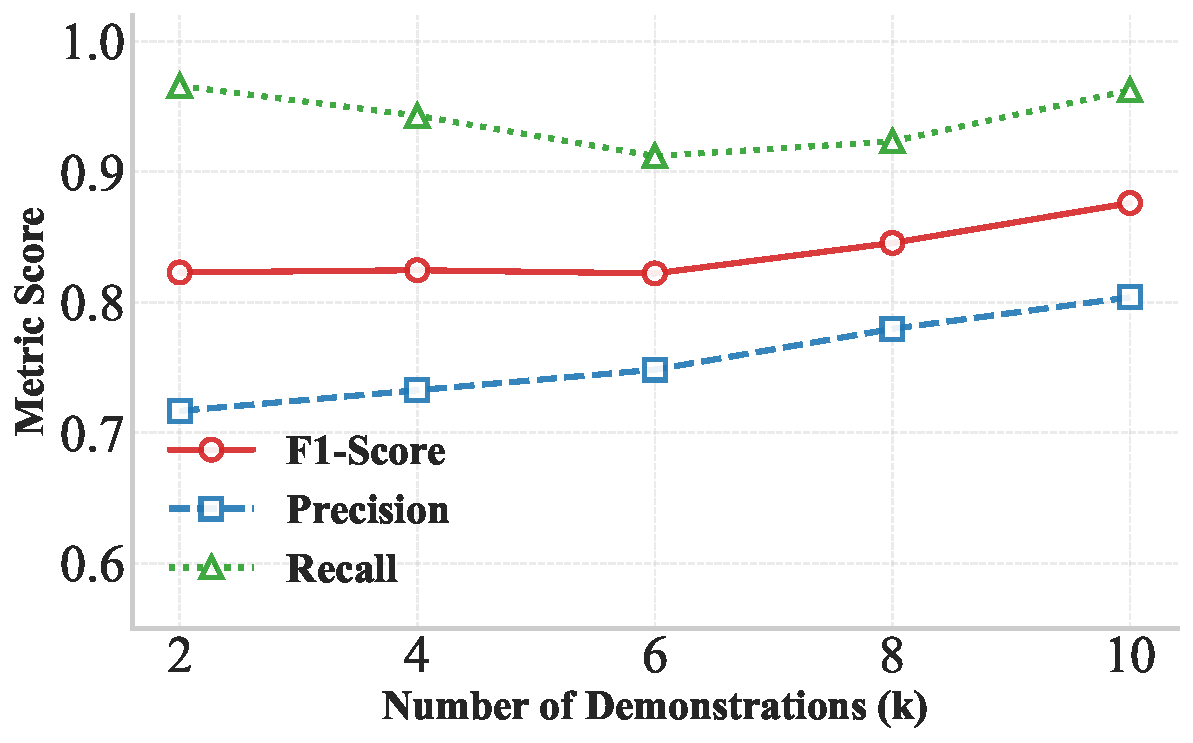
\includegraphics[width=0.4\textwidth]{Figures/BTT_15k_sensitivity_k_metrics_bold_offset.pdf}
        \label{fig:btt}
    }
    \hfill % 撑开间距
    % 右上图
    \subfloat[Description for Thunderbird-Liberty]{
        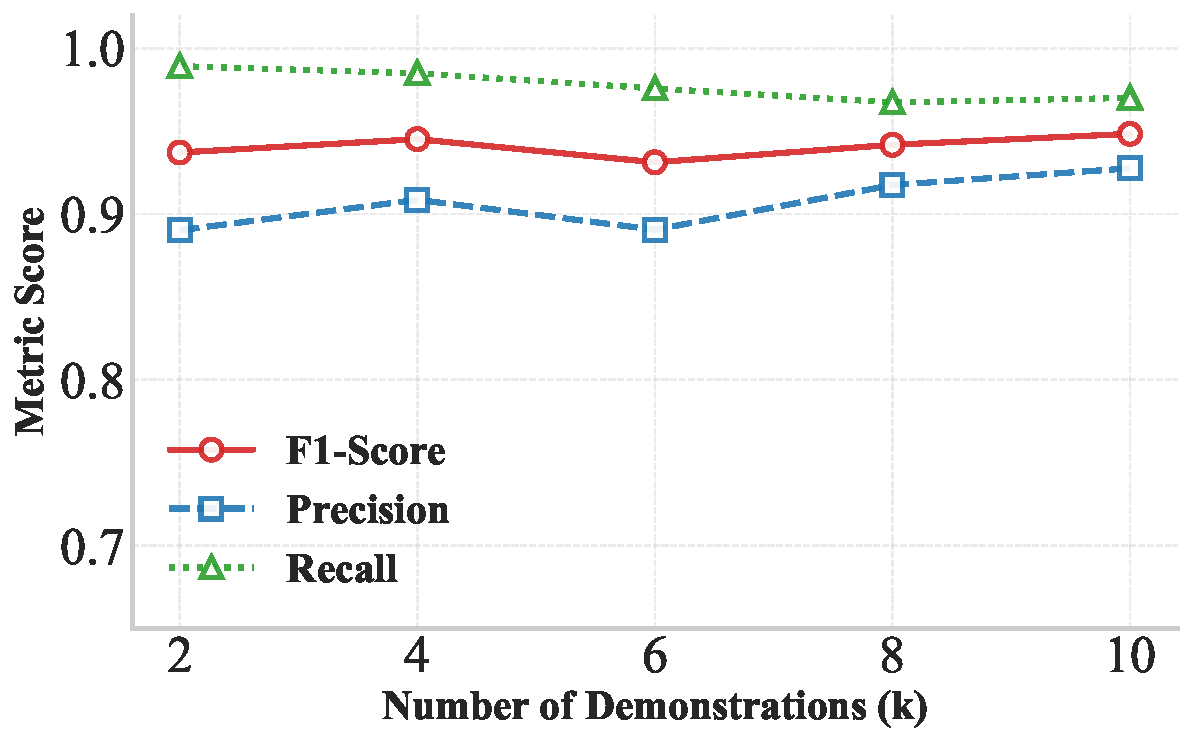
\includegraphics[width=0.4\textwidth]{Figures/TLL_15k_sensitivity_k_metrics_bold_offset.pdf}
        \label{fig:tll}
    }
    
    \vspace{-1em} % 增加行间距
    
    % --- 第二行 ---
    % 左下图
    \subfloat[Description for BGL-Liberty]{
        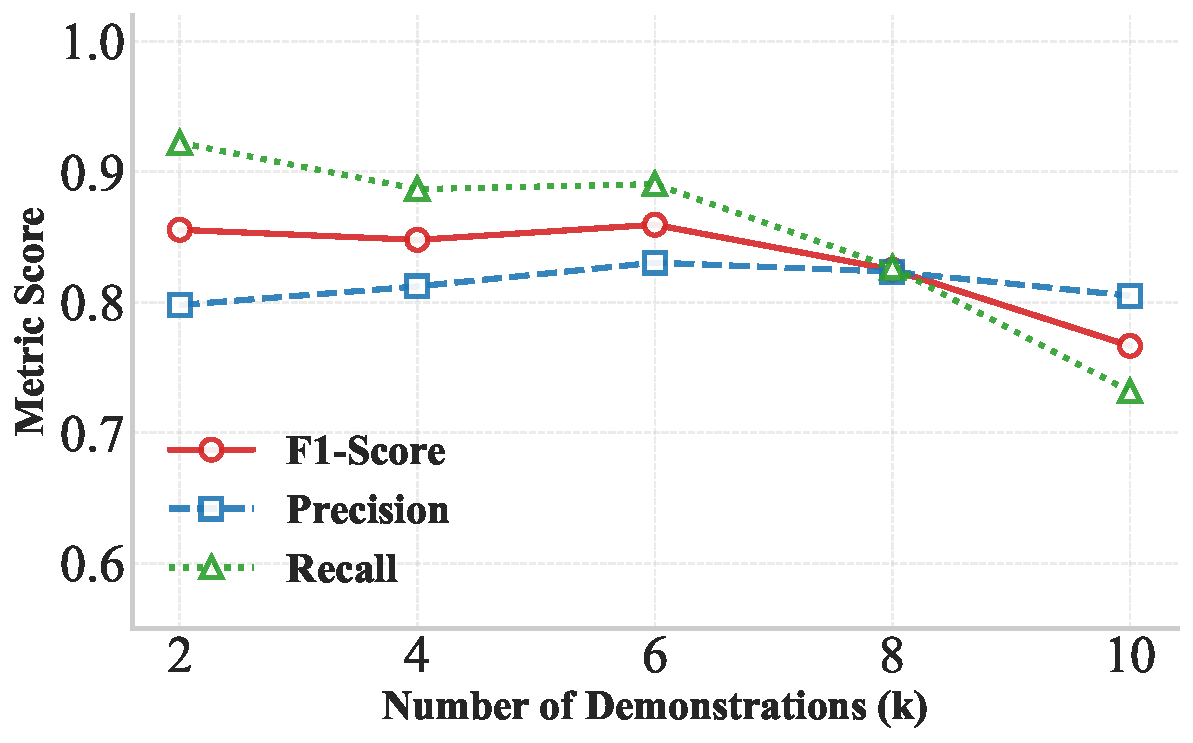
\includegraphics[width=0.4\textwidth]{Figures/BLL_15k_sensitivity_k_metrics_bold_offset.pdf}
        \label{fig:bll}
    }
    \hfill
    % 右下图
    \subfloat[Description for Liberty-BGL]{
        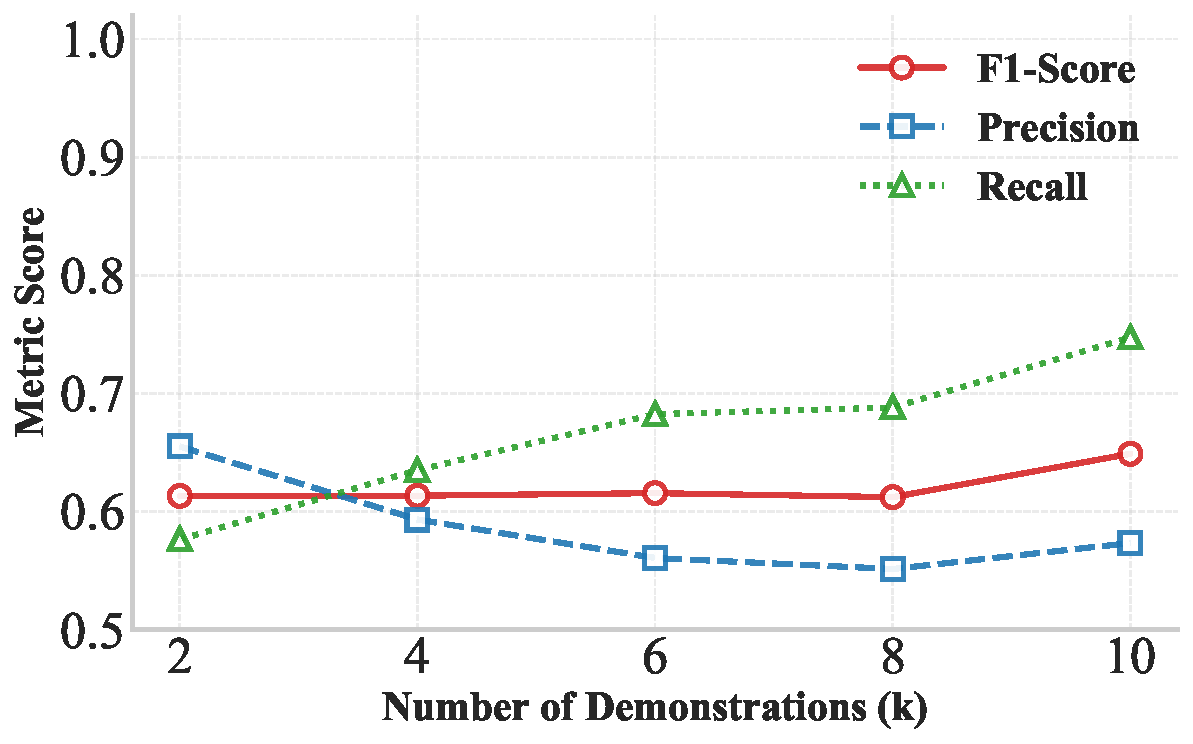
\includegraphics[width=0.4\textwidth]{Figures/LBB_15k_sensitivity_k_metrics_bold_offset.pdf}
        \label{fig:lbb}
    }
    
    \caption{Parameter sensitivity analysis across four different metrics.}
    \label{fig:parameter_sensitivity_all}
\end{figure*}




\begin{table}[t]
    \centering
    \small % 保持小号字体
    \setlength{\tabcolsep}{6pt} % 保持列间距
    
    % 保持标题样式为小型大写 + 无句号
    \caption{\textsc{Ablation Study on Loss Components.}}
    \label{tab:ablation_loss}
    
    \begin{tabular}{@{} c c c c @{}} 
    \toprule
    % 修改处：[-3pt] 表示将文字向下移动 3pt，使其在视觉上垂直居中
    \multirow{2}{*}[-3pt]{\textbf{Transfer Task}} & \multicolumn{3}{c}{\textbf{F1-Score (\%)}} \\
    \cmidrule(l){2-4}
    & \textbf{w/o Opt} & \textbf{w/o ICL-Guided} & \textbf{LogICL} \\
    \midrule
    
    Liberty-BGL & 23.73 & 38.11 & \textbf{74.04} \\
    BGL-Thunderbird & 39.58 & 79.56 & \textbf{89.32} \\
    BGL-Liberty & 59.35 & 73.49 & \textbf{79.56} \\
    Thunderbird-Liberty & 71.95 & 83.65 & \textbf{85.20} \\
    
    \bottomrule
    \end{tabular}
\end{table}


% \begin{table}[t]
%     \centering
%     \small % 保持小号字体
%     \setlength{\tabcolsep}{6pt} % 适当调整列间距，使其紧凑但易读
%     % 移除 arraystretch 或设为 1.0，以消除不必要的垂直稀疏感
    
%     \caption{\textsc{ABLATION STUDY ON LOSS COMPONENTS}}
%     \label{tab:ablation_loss}
    
%     % 使用标准 tabular (l c c c) 结构，防止表格被拉伸
%     \begin{tabular}{@{} l c c c @{}} 
%     \toprule
%     \multirow{2}{*}{\textbf{Transfer Task}} & \multicolumn{3}{c}{\textbf{F1-Score (\%)}} \\
%     \cmidrule(l){2-4}
%     % 使用缩写：w/o Opt. (w/o Optimization); w/o ICL (w/o ICL-Guided)
%     & \textbf{w/o Opt.} & \textbf{w/o ICL} & \textbf{LogICL} \\
%     \midrule
    
%     Liberty-BGL & 55.4 & 68.2 & \textbf{74.2} \\
%     BGL-Thunderbird & 65.2 & 76.5 & \textbf{82.5} \\
%     BGL-Liberty & 61.3 & 72.8 & \textbf{79.4} \\
%     Thunderbird-Liberty & 60.8 & 71.5 & \textbf{78.6} \\
    
%     \bottomrule
%     \end{tabular}
% \end{table}

% \subsection{Ablation Study}

% To validate the effectiveness of our proposed multi-objective loss and ICL-Guided Loss, we conducted ablation studies as presented in Table~\ref{tab:ablation_loss}. We compare the complete LogICL framework against two variants: (1) \textit{w/o Opt} (without optimization), which employs a frozen encoder, and (2) \textit{w/o ICL-Guided} (without ICL-Guided Loss), which excludes only the $L_{\text{Delta}}$ component.

% The results demonstrate that the \textit{w/o Opt} setting yields the lowest performance across all tasks (e.g., 55.4\% on Liberty-BGL). This degradation confirms that a frozen encoder, relying solely on raw pre-trained knowledge, lacks the capability for domain alignment and task-specific feature extraction, making it ineffective for cross-system transfer. 
% Furthermore, while the \textit{w/o ICL-Guided} variant improves upon the frozen baseline via basic domain adaptation, it still underperforms the full model. Without the supervision of $L_{\text{Delta}}$, the encoder fails to capture the latent semantic equivalence preferred by the LLM for reasoning. Instead, it regresses to identifying demonstrations based on surface lexical similarity among samples with identical labels, which is less robust for in-context learning. The superior performance of the full LogICL framework validates that integrating all objectives is essential for bridging the semantic gap in cross-domain log analysis.

\subsection{Ablation Study}
To verify the contribution of each proposed component, we conduct comprehensive ablation studies on the multi-objective optimization and the ICL-Guided Loss, with results reported in Table~\ref{tab:ablation_loss}. We compare the complete LogICL framework against two ablated variants: (1) \textit{w/o Opt}, which freezes the log encoder and relies solely on the raw pre-trained representation without any optimization, and (2) \textit{w/o ICL-Guided}, which removes only the $L_{\text{Delta}}$ component while retaining the other training objectives.

As shown in Table~\ref{tab:ablation_loss}, the \textit{w/o Opt} variant exhibits dramatically lower performance across all transfer tasks, achieving only 23.73\% F1 on Liberty-BGL—the most challenging cross-system transfer—and at most 71.95\% F1 on the relatively easier Thunderbird-Liberty transfer. This sharp degradation underscores that a frozen encoder, even when pre-trained on massive log data, cannot effectively bridge the substantial domain gap between different logging systems without explicit alignment and task-adaptive fine-tuning.

Removing only the ICL-Guided Loss (\textit{w/o ICL-Guided}) yields substantial gains over the frozen baseline (e.g., +14.38 points on Liberty-BGL and +39.98 points on BGL-Thunderbird), demonstrating the benefit of basic contrastive domain adaptation. Nevertheless, this variant still lags considerably behind the full LogICL model, with gaps ranging from 11.55 to 35.93 F1 points across tasks. The most pronounced drop occurs on the Liberty-BGL transfer (38.11\% vs. \textbf{74.04\%}), highlighting that, without the explicit supervision from $L_{\text{Delta}}$, the encoder tends to capture superficial lexical patterns or source-system biases rather than the deeper semantic invariants that the LLM actually leverages during in-context reasoning.

The full LogICL framework, which jointly optimizes all objectives, consistently achieves the highest performance, reaching 74.04\%–89.32\% F1 across diverse cross-system transfers. These results conclusively validate that both trainable domain-adaptive optimization and the ICL-Guided semantic alignment signal are indispensable for narrowing the modality and distribution gap between structured log representations and the LLM’s in-context learning mechanism. The synergistic integration of these components is the key to robust and generalizable cross-system log anomaly detection.

%----------------------------------------------------------------------------------


% 使用 figure* 环境使图片横跨两栏
\begin{figure*}[htbp]
    \centering
    
    % --- 第一行 (Row 1) ---
    \begin{minipage}[t]{0.49\textwidth} % 左图，占据页面宽度约49%
        \centering
        % 使用 width=\linewidth 确保图片填满 minipage 的宽度
        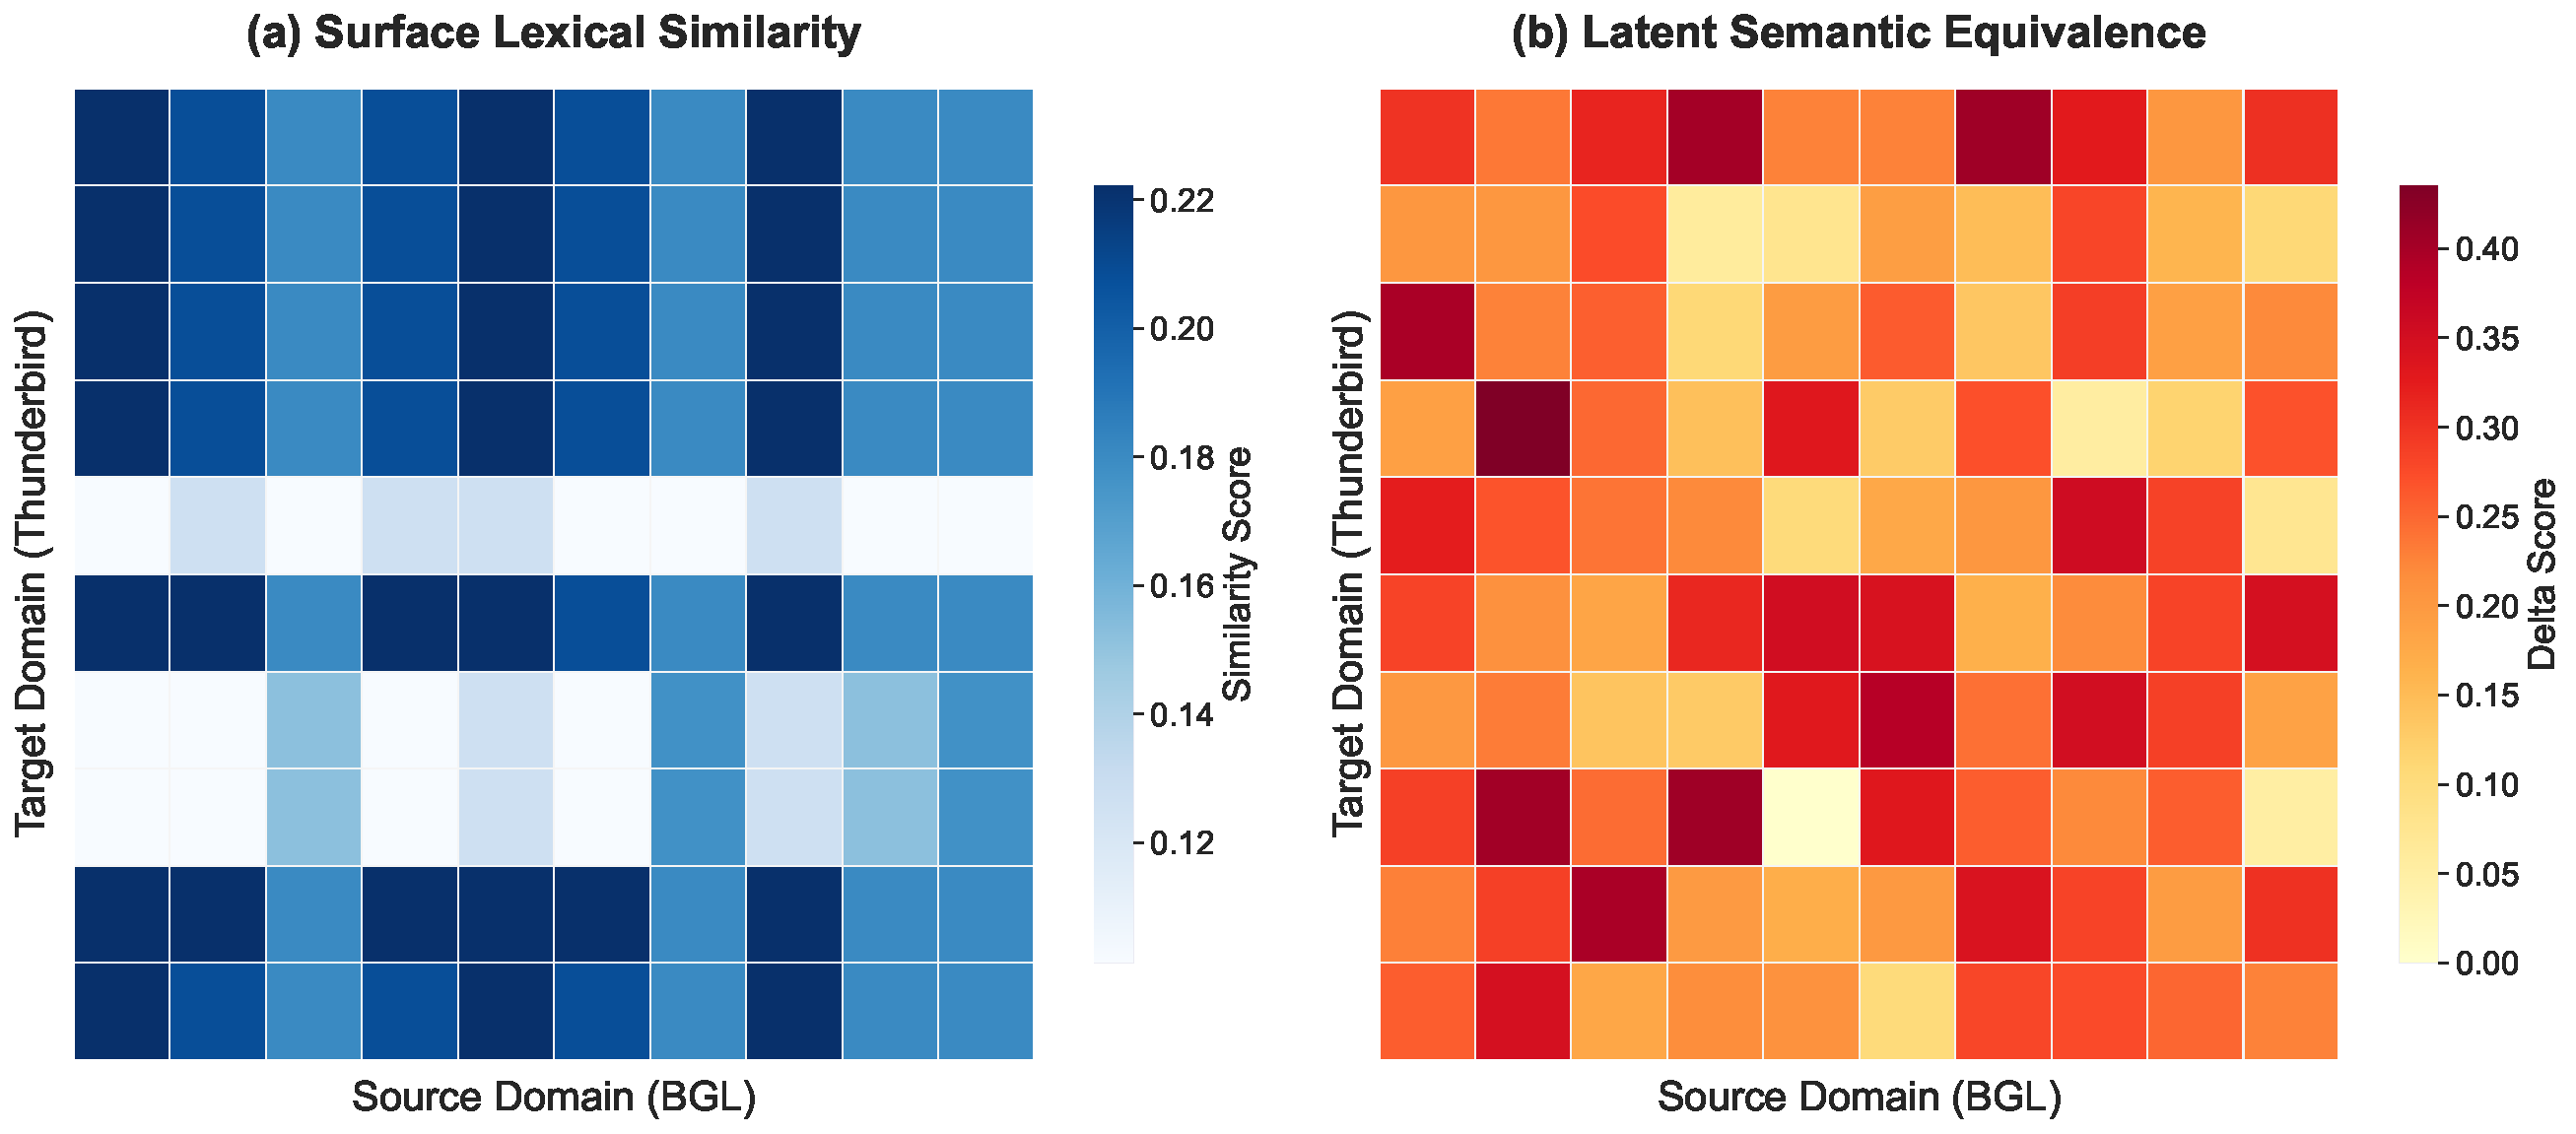
\includegraphics[width=\linewidth]{Figures/new_big_BTT_case_study_comparison.pdf} 
        \vspace{2pt}
        \centerline{\footnotesize (a) BTT Transfer} % 建议加上子图标签
    \end{minipage}
    \hfill % 填充中间的空白空间
    \begin{minipage}[t]{0.49\textwidth} % 右图，占据页面宽度约49%
        \centering
        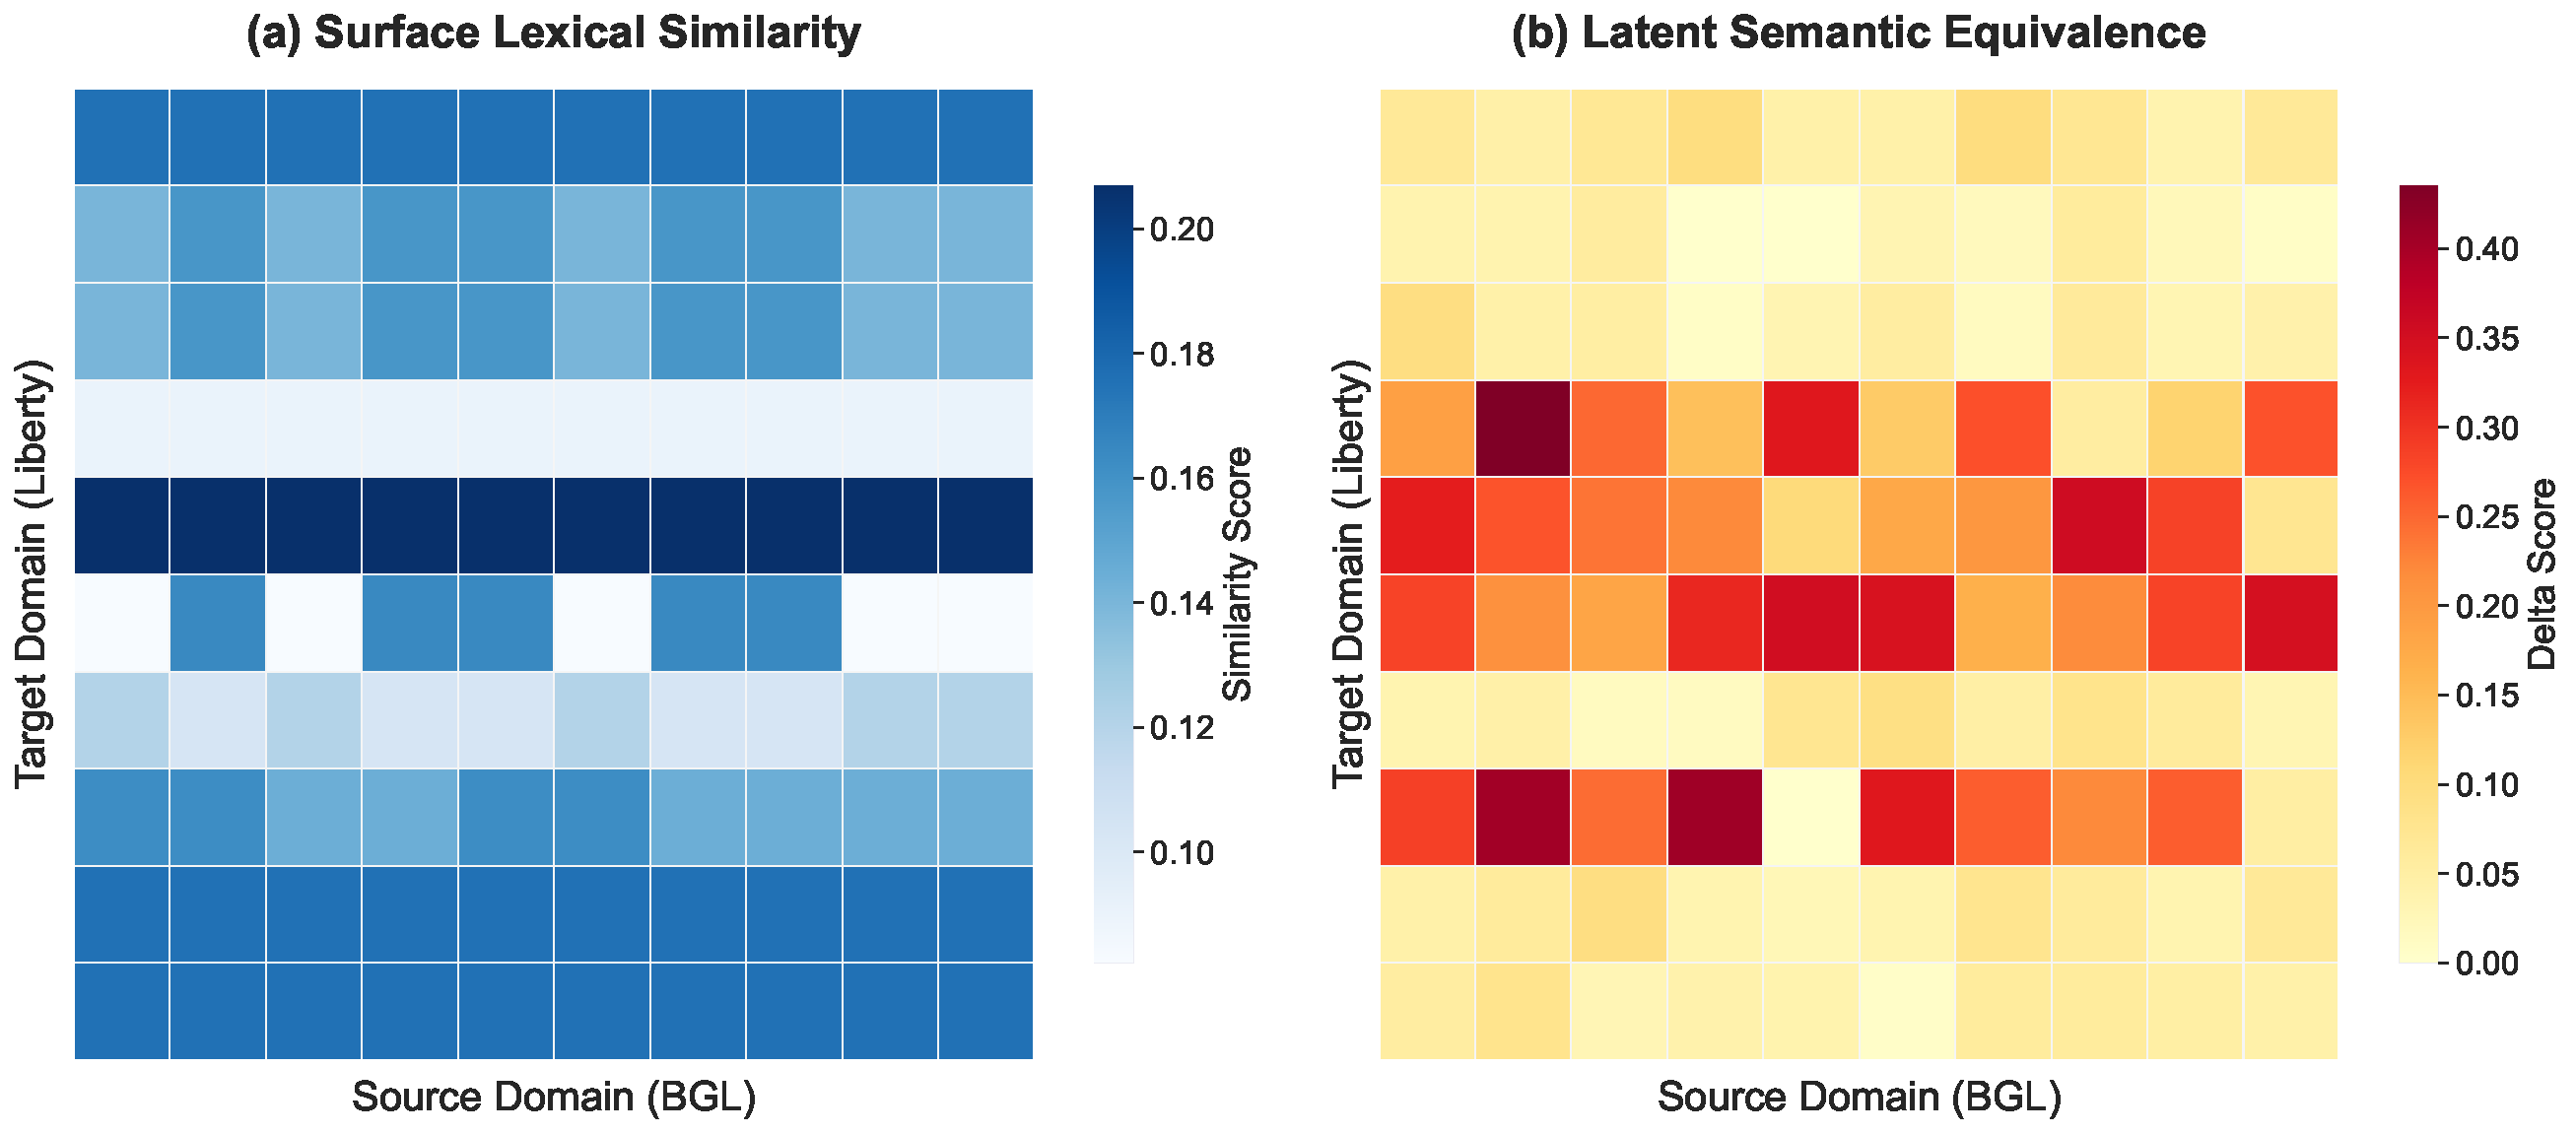
\includegraphics[width=\linewidth]{Figures/new_big_BLL_case_study_comparison.pdf}
        \vspace{2pt}
        \centerline{\footnotesize (b) BLL Transfer} % 建议加上子图标签
    \end{minipage}
    
    % 在两行之间增加一些垂直间距，让图片不至于挤在一起
    \vspace{4mm}
    
    % --- 第二行 (Row 2) ---
    \begin{minipage}[t]{0.49\textwidth} % 左图
        \centering
        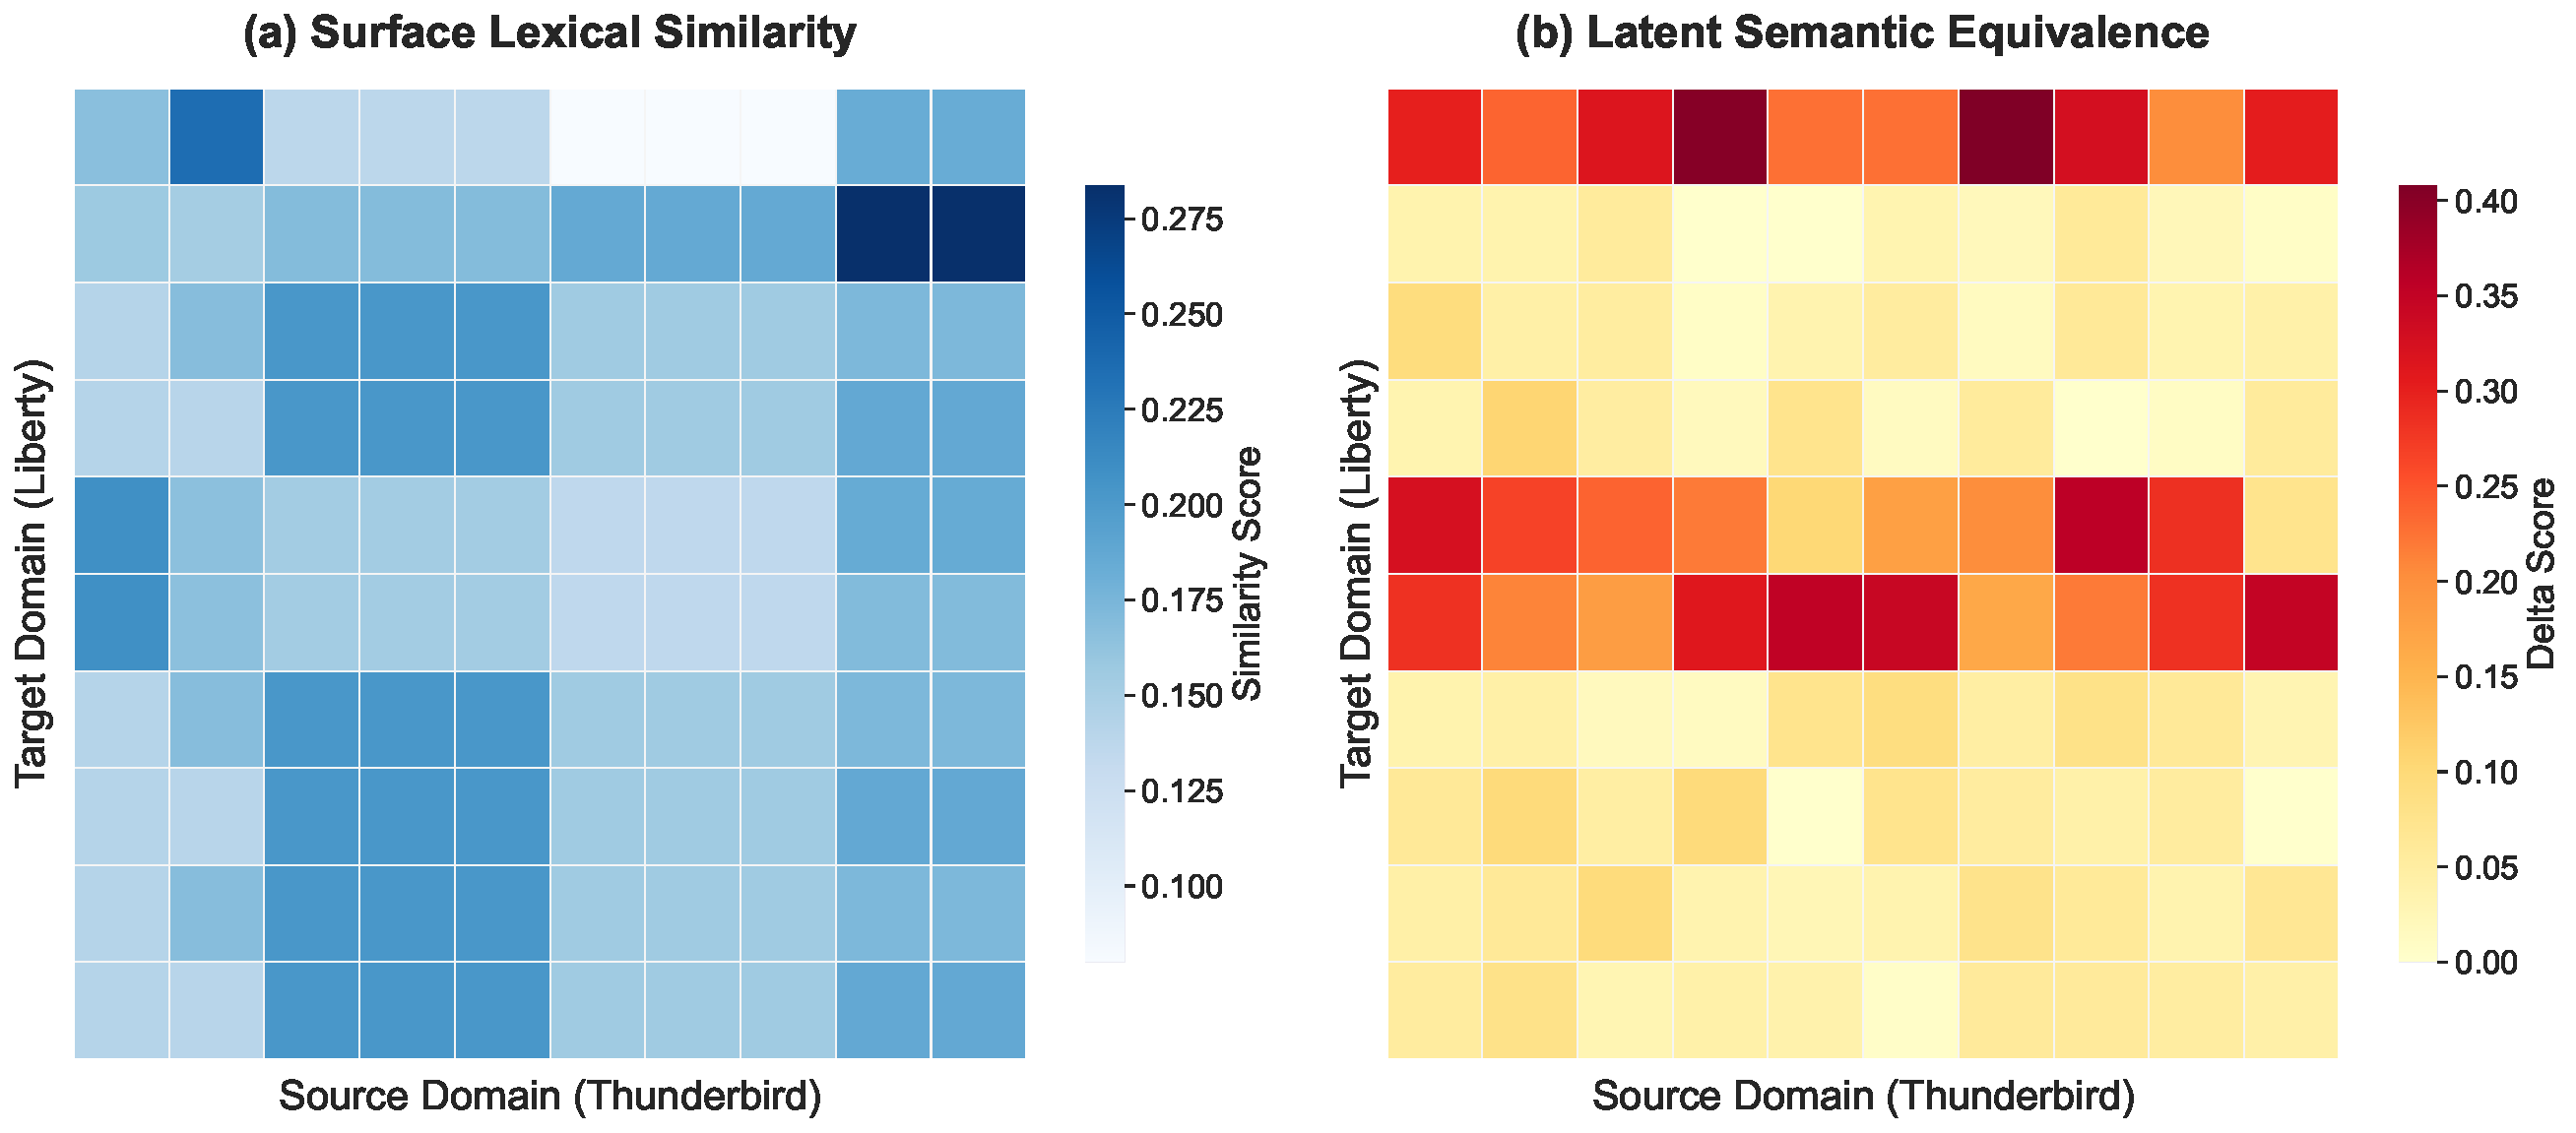
\includegraphics[width=\linewidth]{Figures/new_big_TLL_case_study_comparison_fixed.pdf}
        \vspace{2pt}
        \centerline{\footnotesize (c) TLL Transfer} % 建议加上子图标签
    \end{minipage}
    \hfill
    \begin{minipage}[t]{0.49\textwidth} % 右图
        \centering
        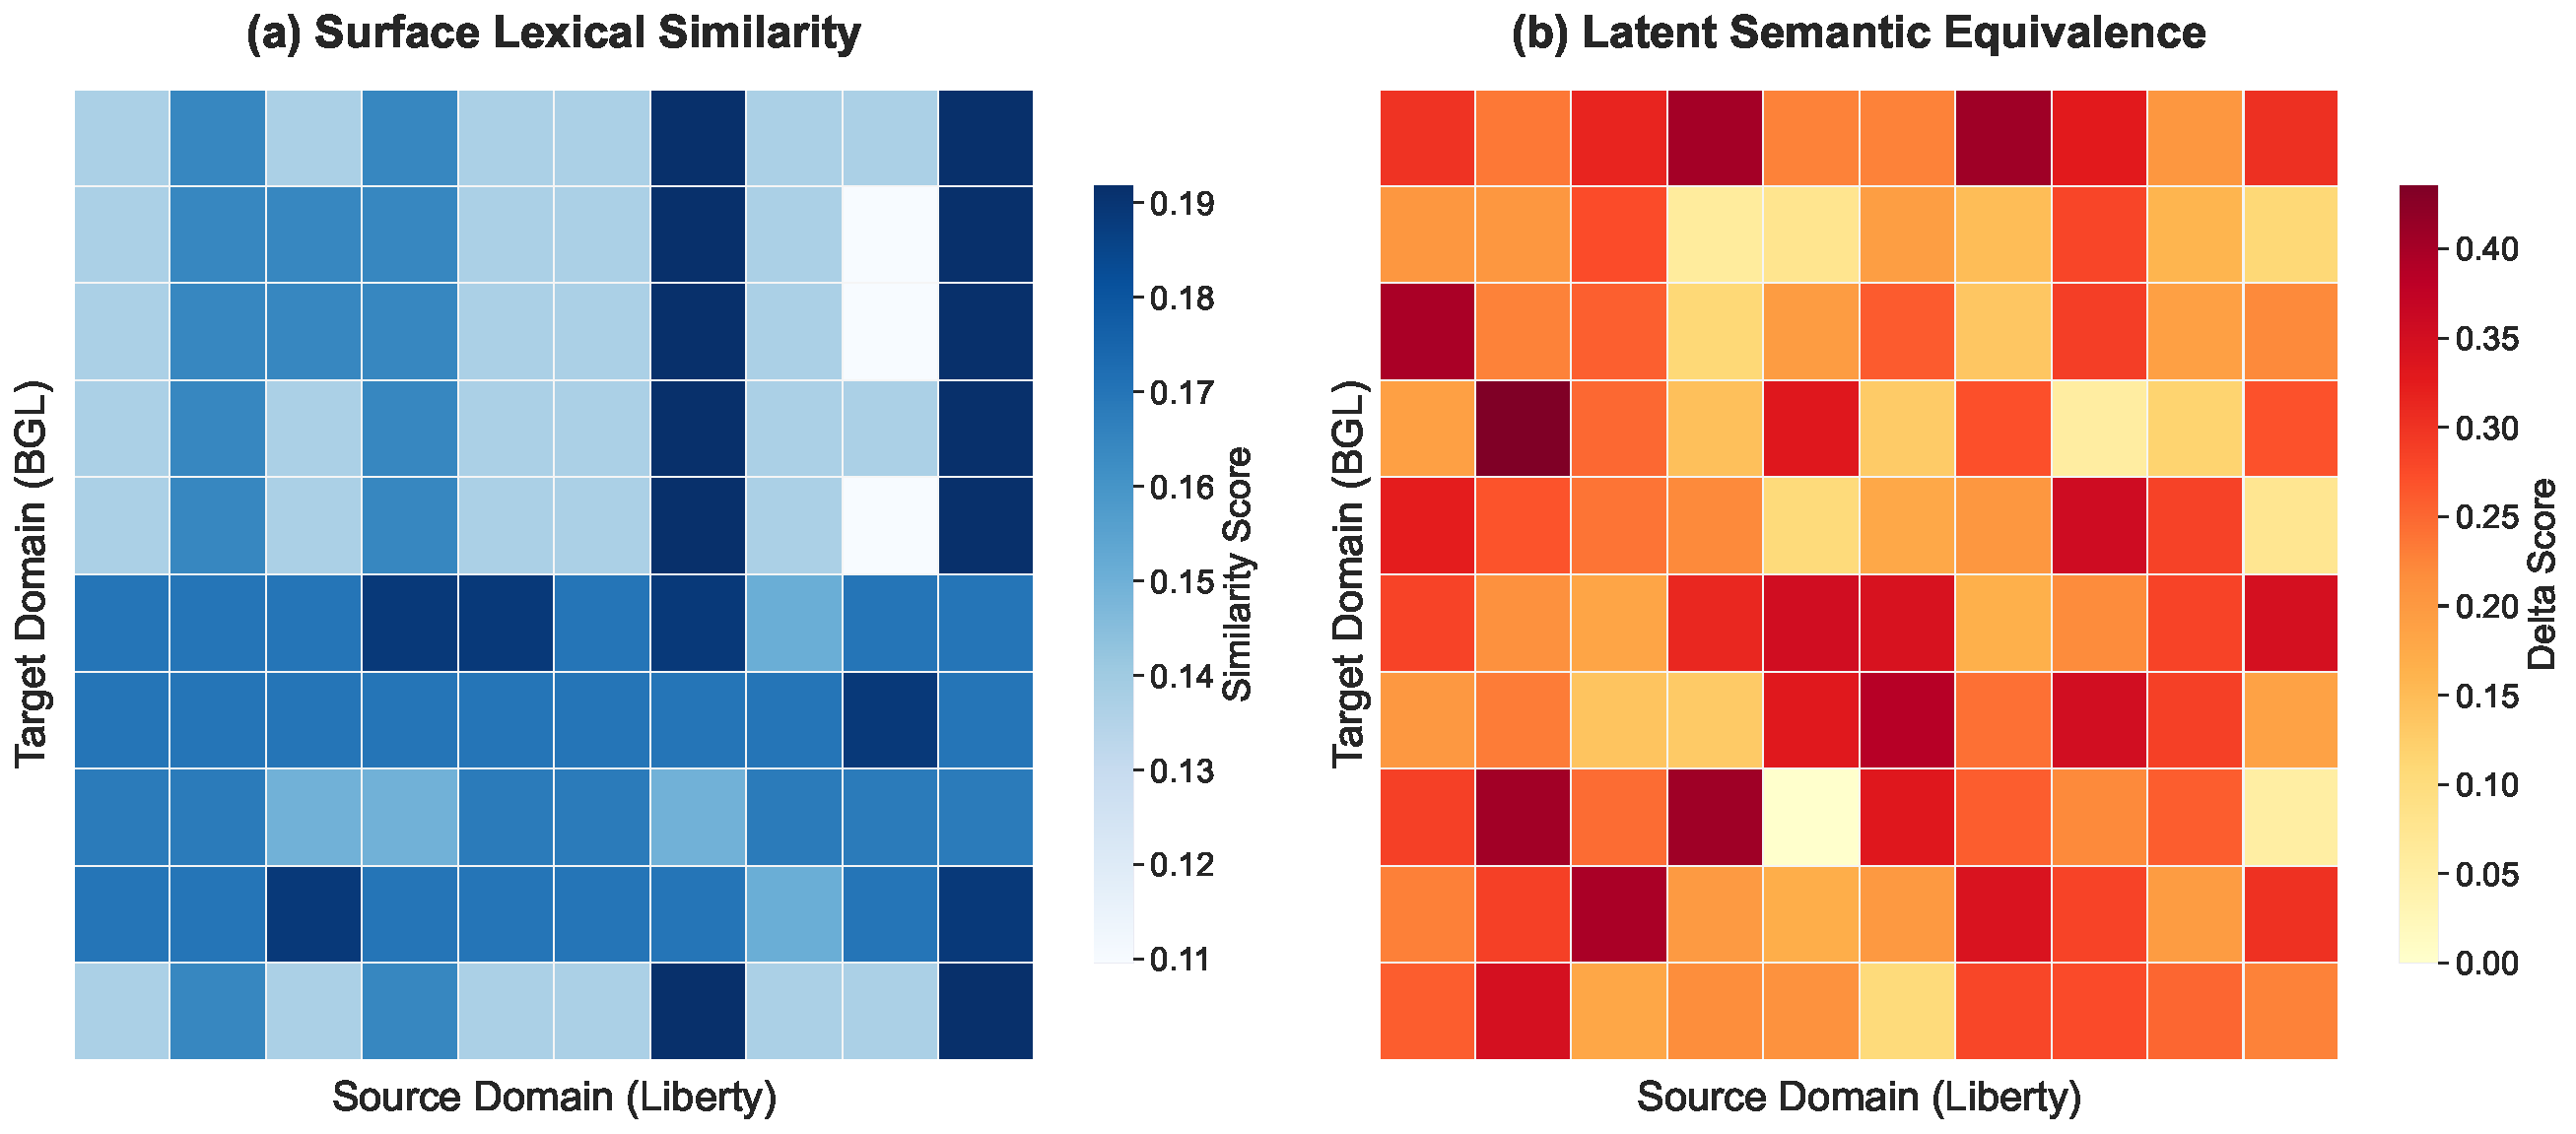
\includegraphics[width=\linewidth]{Figures/new_big_LBB_case_study_comparison.pdf}
        \vspace{2pt}
        \centerline{\footnotesize (d) LBB Transfer} % 建议加上子图标签
    \end{minipage}
    
    % 统一的图标题和标签
    \caption{\textbf{Visualization of Alignment Mechanisms.} 
    Comparison between surface lexical similarity (blue, left) and Latent Semantic Equivalence (red, right) across (a) BTT, (b) BLL, (c) TLL, and (d) LBB scenarios. 
    The contrast highlights LogICL's ability to overcome vocabulary mismatches by capturing deep \textbf{semantic equivalence} and \textbf{structural homology} (e.g., matching error burst patterns), confirming that demonstrations serve as effective structural prototypes.}
    \label{fig:Visualization of Alignment Mechanisms} % 建议更改标签以避免与之前的 \label{fig} 重复
\end{figure*}


\subsection{Interpretability of Alignment Mechanisms}

To empirically validate the interpretability of LogICL, we visualize the alignment mechanisms across four cross-domain scenarios. As illustrated in Figure \ref{fig:Visualization of Alignment Mechanisms}, in these heatmaps, the x-axis represents samples from the source domain, and the y-axis represents samples from the target domain. Each cell quantifies the pairwise relationship between a source-target pair using two distinct metrics: Surface Lexical Similarity (Blue Matrices, calculated via cosine similarity) and Latent Semantic Equivalence (Red Matrices, it is also the delta matrix).

\subsubsection{Lexical Disparity (Blue Matrices)}
As shown in the blue heatmaps, the overall color distribution is predominantly light, indicating consistently low cosine similarity scores across most cross-domain pairs. This visual evidence confirms a severe lexical disparity: the distinct system environments (e.g., BGL vs. Liberty) share negligible vocabulary overlap, rendering traditional keyword-based retrieval methods ineffective as they fail to find relevant neighbors in the source domain.

\subsubsection{Semantic Equivalence (Red Matrices)}
In contrast, the red heatmaps exhibit distinct clusters of dark red regions (high delta scores). These ``hot spots" indicate that despite the low lexical similarity, specific source demonstrations make significant contributions to the model's reasoning process. This discrepancy captures deep semantic equivalence, where LogICL successfully identifies source logs that are textually distinct but functionally analogous to the target logs. The retrieved demonstrations act as structural prototypes, guiding the LLM to perform robust inductive reasoning beyond superficial keyword matching.
%----------------------------------------------------------------------------------

\begin{table*}[t]
    \centering
    \small
    % 【修改点2】将行高从 1.5 改为 1.2，使整体更紧凑
    \renewcommand{\arraystretch}{1.2} 
    
    % 保持垂直居中设置
    \renewcommand{\tabularxcolumn}[1]{m{#1}}
    
    % 标题建议加上 \textsc 保持顶会风格的小型大写
    \caption{\textsc{Qualitative Analysis: Bridging Surface Lexical Gaps via Latent Semantic Alignment.}} 
    \label{tab:case_study}
    
    % 【关键修改点】
    % 第3列原为 m{3cm}，改为 >{\centering\arraybackslash}m{3cm} 以实现居中
    \begin{tabularx}{\textwidth}{@{} 
        >{\centering\arraybackslash}m{2.5cm}   % Role (居中)
        >{\raggedright\arraybackslash}X        % Log Sequence (左对齐)
        >{\centering\arraybackslash}m{3cm}     % Surface Semantics (居中 - 已修改)
        m{4.5cm}                               % Latent Alignment (左对齐，因为包含列表，左对齐通常更整齐)
    @{}}
    \toprule
    \textbf{Role} & \textbf{Log Sequence Context} & \textbf{Surface Semantics} & \textbf{Latent Alignment} \\
    \midrule
    
    % --- Row 1: Target Input ---
    \textbf{Target Domain} (BGL) & 
    generating core.2516 ;-; generating core.2517 ;-; generating core.2380 ;-; generating core.2382 ;-; generating core.2509 ... & 
    \textbf{Process Crash} \newline \textcolor{gray}{(Memory Context)} & 
    
    % 右侧跨行
    \multirow{2}{=}{%
        \textbf{Mechanism:}\par
        1. \textbf{Resource Exhaustion}\newline
        {\color{gray}\footnotesize (Availability Collapse)}\par
        \vspace{0.5em}
        2. \textbf{Burstiness Pattern}\newline
        {\color{gray}\footnotesize (High-Freq Repetition)}
    } \\
    
    % 分隔线
    \cmidrule(r){1-3}
    
    % --- Row 2: Retrieved Demo ---
    \textbf{Retrieved Demo} (Thundebird) & 
    dhcpd: DHCPDISCOVER from ... network 172.30.0/16: \textcolor{red}{no free leases} ;-; dhcpd: DHCPDISCOVER from ... network 172.31.0/16: \textcolor{red}{no free leases} ... & 
    \textbf{Alloc. Failure} \newline \textcolor{gray}{(Network Context)} & 
    \\ 
    
    \bottomrule
    \end{tabularx}
\end{table*}

% \begin{table*}[t]
%     \centering
%     \small
%     % 【修改点2】将行高从 1.5 改为 1.2，使整体更紧凑
%     \renewcommand{\arraystretch}{1.2} 
    
%     % 保持垂直居中设置
%     \renewcommand{\tabularxcolumn}[1]{m{#1}}
    
%     \caption{Qualitative Analysis: Bridging Surface Lexical Gaps via Latent Semantic Alignment.} 
%     \label{tab:case_study}
    
%     % 【修改点1】X列定义修改：
%     % 原代码：>{\ttfamily\footnotesize\raggedright\arraybackslash}X 
%     % 新代码：>{\raggedright\arraybackslash}X
%     % 去掉了 \ttfamily (打字机字体) 和 \footnotesize (小字号)，现在字体大小和格式与其他列完全一致
%     \begin{tabularx}{\textwidth}{@{} >{\centering\arraybackslash}m{2.5cm} >{\raggedright\arraybackslash}X m{3cm} m{4.5cm} @{}}
%     \toprule
%     \textbf{Role} & \textbf{Log Sequence Context} & \textbf{Surface Semantics} & \textbf{Latent Alignment} \\
%     \midrule
    
%     % --- Row 1: Target Input ---
%     \textbf{Target Domain} (BGL) & 
%     generating core.2516 ;-; generating core.2517 ;-; generating core.2380 ;-; generating core.2382 ;-; generating core.2509 ... & 
%     \textbf{Process Crash} \newline \textcolor{gray}{(Memory Context)} & 
    
%     % 右侧跨行
%     \multirow{2}{=}{%
%         \textbf{Mechanism:}\par
%         1. \textbf{Resource Exhaustion}\newline
%         {\color{gray}\footnotesize (Availability Collapse)}\par
%         % 因为行高变紧凑了，这里的间距也要相应从 1.5em 减小到 0.5em，否则会撑破单元格
%         \vspace{0.5em}
%         2. \textbf{Burstiness Pattern}\newline
%         {\color{gray}\footnotesize (High-Freq Repetition)}
%     } \\
    
%     % 分隔线
%     \cmidrule(r){1-3}
    
%     % --- Row 2: Retrieved Demo ---
%     \textbf{Retrieved Demo} (Thundebird) & 
%     dhcpd: DHCPDISCOVER from ... network 172.30.0/16: \textcolor{red}{no free leases} ;-; dhcpd: DHCPDISCOVER from ... network 172.31.0/16: \textcolor{red}{no free leases} ... & 
%     \textbf{Alloc. Failure} \newline \textcolor{gray}{(Network Context)} & 
%     \\ 
    
%     \bottomrule
%     \end{tabularx}
% \end{table*}

\subsection{Case study}
To validate the effectiveness of our delta-guided retrieval mechanism, we analyze a representative high-delta pair identified during inference. This pair shows minimal lexical overlap ($similarity<0.1$) yet provides a strong positive contribution to detection accuracy ($\delta > 0.8$). As illustrat in Table~\ref{tab:case_study}, the target domain sequence BGL contains repeated \textit{generating core} events indicating persistent process crashes, while the retrieved demonstration from the Thunderbird consists mainly of \textit{dhcpd: no free leases} errors. Despite their distinct vocabularies, the model establishes meaningful semantic alignment and structural correspondence between the two domains. Semantically, both sequences describe a form of \textit{Resource Exhaustion}: the target reflects system context failure, and the source reflects address pool depletion. Structurally, the demonstration illustrates a typical \textit{Burstiness Pattern} (high-frequency repetition indicates a system infinite loop or a retry storm), allowing the model to learn through in-context examples that frequent repetition of a critical error signals a system-level anomaly. This case indicates that our multi-objective loss encourages the model to move beyond keyword matching and supports robust reasoning across heterogeneous system environments.


% \subsection{Threats to Validity}
% While LogICL demonstrates superior performance over existing baselines in cross-domain few-shot and zero-shot settings by optimizing demonstration retrieval, we acknowledge two primary threats to the validity and generalization of our findings. 
% First, the inference accuracy of LLMs remains highly sensitive to Prompt Engineering. Although our method provides optimal demonstrations, the final reasoning quality is inevitably coupled with the design of instruction templates; as evidenced by prior works like LogPrompt, suboptimal or ambiguous instructional phrasing can significantly degrade performance, potentially overshadowing the gains from high-quality demonstrations. 
% Second, there remains a cognitive gap between a general-purpose LLM (e.g., Qwen-14B) equipped with ICL and a true AIOps Expert. While LogICL enhances the model's ability to emulate expert behavior via context, it does not fundamentally alter the model's intrinsic parameters. To achieve human-level reliability in complex system diagnosis, future iterations may require injecting professional operations knowledge at the source—leveraging domain-specific fine-tuning or Reinforcement Learning from Human Feedback (RLHF)—to cultivate an implicit Chain-of-Thought that mimics the deductive reasoning process of seasoned reliability engineers.

% Despite LogICL's strong performance, several threats to validity must be acknowledged.
% First, prompt sensitivity remains a critical limitation in LLM-based inference. Even with optimally retrieved demonstrations, anomaly detection accuracy is highly dependent on prompt wording and template design. As shown in prior work~\cite{liu2024logprompt}, poorly crafted instructions can introduce substantial variance, potentially masking the benefits of high-quality in-context examples.
% Second, limited model capacity constrains few-shot and zero-shot effectiveness. Our inference relies on a 14B-parameter LLM (Qwen-14B), far smaller than the 175B-scale models where robust in-context learning was first shown to emerge~\cite{brown2020language}. On complex or subtle log anomaly patterns—especially those involving long-range dependencies or rare event sequences—smaller models exhibit reduced ability to fully exploit demonstrations, resulting in suboptimal generalization compared to frontier-scale LLMs.
% Third, the gap between general-purpose LLMs and AIOps expertise persists. While LogICL improves contextual reasoning, it does not endow the model with deep operational knowledge or structured diagnostic reasoning. Achieving expert-level performance on multi-cause, temporally extended, or highly ambiguous anomalies will likely require domain-specific fine-tuning or reinforcement learning from human feedback (RLHF) to internalize reliable chain-of-thought patterns typical of experienced reliability engineers.
% These limitations highlight meaningful avenues for future work while situating LogICL as a significant step toward scalable and generalizable log anomaly detection.

\subsection{Threats to Validity}
We acknowledge three primary factors that may impact the validity and generalization of our findings.

\textbf{Sensitivity to Prompt Design.} The inference accuracy of ICL is contingent upon the quality of instruction templates. As instructional ambiguity can act as a confounding variable, suboptimal prompt engineering may potentially mask the performance gains attributed to our demonstration retrieval mechanism.

\textbf{Gap between Frozen LLMs and Domain Expertise.} While LogICL effectively bridges semantic gaps via context, general-purpose LLMs lack intrinsic AIOps expertise. Since our approach operates without parameter updates, the model's deductive reasoning is bounded by its pre-trained knowledge. Achieving human-level reliability in complex diagnostics may necessitate integrating explicit domain adaptation strategies, such as fine-tuning or Reinforcement Learning from Human Feedback (RLHF).

\textbf{Impact of Model Scale.} As established by Brown et al.~\cite{brown2020language}, few-shot ICL is an emergent ability that scales significantly with model size. Our deployment of a moderate-sized model (14B)—chosen to balance computational efficiency—may not fully unlock the peak reasoning potential observed in larger foundation models (e.g., 175B), representing a necessary trade-off between resource constraints and optimal few-shot performance.

\section{Discussion}
\textbf{Metrics vs. Reality: The Anomaly Discovery Gap} Our error analysis on the BGL dataset initially indicated a high false positive rate; however, manual inspection revealed that these instances were largely latent anomalies mislabeled as normal in the ground truth. This discrepancy highlights the susceptibility of traditional supervised baselines to overfitting label noise within closed-world training data. In contrast, LogICL leverages the intrinsic semantic knowledge of frozen LLMs to identify generic anomaly patterns (e.g., system failures) that contradict noisy annotations. We validated this capability by refining the BGL dataset based on criteria from prior work~\cite{xu2025rationanomaly}, demonstrating that LogICL functions effectively as a robust zero-shot ``Data Auditor.'' These findings underscore the critical impact of label quality and urge future research to prioritize dataset reliability alongside performance metrics.
% \textbf{Metrics vs. Reality: The Anomaly Discovery Gap}. A critical experimental finding was the initial high rate of false positives on the BGL dataset. However, qualitative analysis revealed that these were largely latent anomalies mislabeled as normal in the ground truth. This discrepancy exposes a fundamental limitation of traditional supervised baselines: they inevitably overfit to label noise within closed-world training data. In contrast, our inference-only LogICL leverages the LLM's vast pre-trained operational knowledge—acquired from massive high-quality corpora—to identify generic anomaly semantics (e.g., system failures) that contradict the noisy specific labels. Consequently, LogICL acts not merely as a detector but as a robust zero-shot Data Auditor, capable of correcting erroneous benchmarks. To solidify this contribution, we refined the BGL dataset by correcting these samples based on established criteria from prior studies \cite{xu2025rationanomaly}, highlighting the critical impact of label quality and urging future research to prioritize dataset reliability alongside model metrics.

\section{Conclusion}
In this paper, we proposed LogICL, a novel cross-domain framework designed to address the cold-start challenge in log anomaly detection by bridging the gap between surface lexical similarity and latent semantic equivalence. Unlike traditional transfer learning methods constrained by static embeddings or data-intensive Transformer adaptations, LogICL distills the reasoning capabilities of LLMs into a lightweight encoder via a novel delta matrix and multi-objective optimization. This approach enables the retrieval of reasoning-aware demonstrations that facilitate effective ICL with a frozen LLM. Extensive experiments on cross-system benchmarks demonstrate that LogICL achieves state-of-the-art performance in both few-shot and zero-shot settings, outperforming existing baselines. 
By combining robust generalization with Chain-of-Thought traceability for enhanced diagnostic insights, LogICL offers a resource-efficient solution for rapid deployment in evolving IT infrastructures.
% By combining robust generalization with Chain-of-Thought interpretability, LogICL offers a resource-efficient solution for rapid deployment in evolving IT infrastructures.

\section*{Acknowledgments}



\bibliographystyle{IEEEtran}
\bibliography{references}{
}

\end{document}


